% ============================================================================
% APPENDIX UN: FORMAL-UNTCM - Unified Natural Trajectory Model
% ============================================================================
% Category: FORMAL (Mathematical Formalization)
% Version: 1.0
% Last Updated: 2026-01-20
% Dependencies: PBB (Probability), V (Context), AAA (WHO), AW (STAGE)
% Language: english
% ============================================================================

% ----------------------------------------------------------------------------
% HEADER BLOCK
% ----------------------------------------------------------------------------
% Code: UN
% Category: FORMAL (Mathematical Formalization)
% Title: Unified Natural Trajectory Model (UNTCM)
% Author: EBF Framework
% Status: Active
% Priority: High
% Evidence-Base: 22+ PRO papers, 4 constructive CONTRA papers
% ----------------------------------------------------------------------------

\chapter{FORMAL-UNTCM: Unified Natural Trajectory Model}
\label{app:formal-untcm}

% ============================================================================
% APPENDIX METADATA
% ============================================================================
\begin{tcolorbox}[colback=gray!10!white, colframe=gray!75!black, title=Appendix Metadata]
\begin{tabular}{@{}ll@{}}
\textbf{Code:} & UN \\
\textbf{Category:} & FORMAL (Mathematical Formalization) \\
\textbf{Title:} & Unified Natural Trajectory Model (UNTCM) \\
\textbf{Version:} & 1.2 (January 2026) \\
\textbf{Status:} & Active \\
\textbf{Priority:} & High \\
\textbf{Elements:} & 29 (A5, T6-T8, M1-M5, D1-D2, T2-T3, I1-I4, E1-E3, X1-X5) \\
\textbf{Evidence:} & 28+ PRO papers, 6 constructive CONTRA papers \\
\textbf{Dependencies:} & PBB, V, AAA, AW, C, BBB, HHH, AN \\
\end{tabular}
\end{tcolorbox}

% ============================================================================
% CROSS-REFERENCE MAP
% ============================================================================
\begin{tcolorbox}[colback=blue!5!white,colframe=blue!75!black,title=Cross-Reference Map]
\textbf{Outgoing References:}
\begin{itemize}
    \item \textbf{PBB (FORMAL-PROBABILITY):} Probability axioms P1-P10, NTM foundations (A1-A4, T1-T5)
    \item \textbf{V (CORE-WHEN):} Context vector $\vec{\Psi}$ definition
    \item \textbf{AAA (CORE-WHO):} Welfare hierarchy and stakeholder levels
    \item \textbf{AW (CORE-STAGE):} Behavioral Change Journey (BCJ) phases
    \item \textbf{C (CORE-WHAT):} FEPSDE utility dimensions
    \item \textbf{BBB (CORE-WHERE):} Parameter repository for calibration
    \item \textbf{HHH (METHOD-TOOLKIT):} Emergent 10C intervention vectors
    \item \textbf{AN (METHOD-LLMMC):} LLM Monte Carlo for parameter estimation
\end{itemize}

\textbf{Incoming References:}
\begin{itemize}
    \item Chapter 16 (Natural Trajectory Model): Primary chapter reference
    \item Chapter 17 (Emergent Interventions): Emergent 10C vectors to UNTCM mapping
    \item Chapter 18 (Intervention Timing): Optimal timing from NTM-T8
    \item Chapter 19 (Segmentation): Segment heterogeneity (I4)
    \item Chapter 20 (Portfolio Archetypes): Archetype selection via UNTCM regime
\end{itemize}
\end{tcolorbox}

% ============================================================================
% CHAPTER LINKAGE
% ============================================================================
\begin{tcolorbox}[colback=green!5!white,colframe=green!75!black,title=Chapter Linkage]
\textbf{Primary Chapter:} Chapter 16 (Natural Trajectory Model)

\textbf{Purpose:} This appendix provides the complete mathematical formalization of the Unified Natural Trajectory Model (UNTCM), which integrates:
\begin{itemize}[nosep]
    \item NTM Decay dynamics (Awareness, Willingness, Threshold)
    \item Context Drift dynamics ($\vec{\Psi}$ evolution)
    \item Feedback loops (Behavior $\rightarrow$ Context $\rightarrow$ Decay rates)
\end{itemize}

\textbf{CORE Connection:} UNTCM connects WHEN (Context, V) with STAGE (Journey, AW) by formalizing how context affects trajectory and when tipping points occur.
\end{tcolorbox}

% ============================================================================
% ABSTRACT AND QUICK REFERENCE
% ============================================================================
\begin{abstract}
The Unified Natural Trajectory Model (UNTCM) formalizes the coupled dynamics of individual behavior change (Awareness $A$, Willingness $W$, Threshold $\theta$) and contextual evolution (social norms $\Psi_S$, technology $\Psi_T$, economic conditions $\Psi_E$, institutions $\Psi_I$, culture $\Psi_C$). The model captures three qualitative regimes: (I) Decay-Dominant where behavior naturally declines, (II) Feedback-Dominant where behavior becomes self-sustaining via positive feedback (lock-in), and (III) Oscillatory where boom-bust cycles emerge. The critical tipping point $\bar{B}^* \approx 10-25\%$ determines when interventions can trigger regime transitions. UNTCM provides a unified framework for intervention timing, portfolio design, and long-term outcome prediction.
\end{abstract}

\begin{tcolorbox}[colback=gray!5!white,colframe=gray!75!black,title=Quick Reference]
\textbf{Key Elements (29 total):}
\begin{itemize}[nosep]
    \item \textbf{Core:} A5 (Context-Modulated Decay), T6 (Coupled ODEs), T7 (Phase Diagram), T8 (Timing Rule)
    \item \textbf{Methodology:} M1 (Computational), M2 (Calibration), M3 (Stochastic), M4 (Optimal Control), M5 (Maintenance Cost)
    \item \textbf{Maintenance Definitions:} M5-D1 (Minimal Portfolio), M5-D2 (Portfolio Archetypes), M5-T2 (Cardinality), M5-T3 (Pareto-Frontier)
    \item \textbf{Integration:} I1 (BCJ), I2 (Emergent 10C Vectors), I3 (FEPSDE), I4 (Segments)
    \item \textbf{Empirical:} E1 (Regime Detection), E2 (Tipping Prediction), E3 (Timing Estimation)
    \item \textbf{Extensions:} X1 (Network), X2 (Hysteresis), X3 (Adaptive $\theta$), X4 (Markov-Switching), X5 (Loss Aversion Lock-in)
\end{itemize}

\textbf{Key Equations:}
\begin{itemize}[nosep]
    \item Coupled ODE System: Eq. \ref{eq:untcm-odes}
    \item Tipping Point: $\bar{B}^* = (\lambda_0 A^* + \mu_0 W^*)/(\kappa_S + \kappa_T + \kappa_I)$
    \item Full Specification: Eq. \ref{eq:untcm-full}
\end{itemize}

\textbf{Three Regimes:}
\begin{enumerate}[nosep]
    \item \textbf{Regime I (Decay):} $\lambda, \mu > \kappa \bar{B}_{max}$ $\rightarrow$ Behavior extinction
    \item \textbf{Regime II (Lock-in):} $\kappa \bar{B} > \lambda, \mu$ at critical mass $\rightarrow$ Self-sustaining
    \item \textbf{Regime III (Oscillatory):} Large $\kappa$, heterogeneous $\tau$ $\rightarrow$ Boom-bust cycles
\end{enumerate}
\end{tcolorbox}

% ============================================================================
% FUNDAMENTAL QUESTION
% ============================================================================
% -----------------------------------------------------------------------------
% APPENDIX SCOPE BOX
% -----------------------------------------------------------------------------

\begin{tcolorbox}[
    colback=orange!5!white,
    colframe=orange!75!black,
    title={\textbf{Appendix Scope: Ziel / In-Scope / Out-of-Scope / Constraints}},
    fonttitle=\bfseries
]

\textbf{Ziel (Objective):}
\begin{itemize}[nosep]
    \item How do individual behavioral dynamics (Awareness, Willingness, Threshold decay) and contextual evolution (social norms, technology, institutions) interact to determine when interventions can achieve lasting behavior change versus temporary effects?
\end{itemize}

\textbf{In-Scope:}
\begin{itemize}[nosep]
    \item Fundamental Question
    \item UNTCM Core Theory
    \item Unified NTM-Context Model (UNTCM)
    \item UNTCM Methodology
    \item UNTCM Framework Integration
\end{itemize}

\textbf{Out-of-Scope (delegiert an andere Appendices):}
\begin{itemize}[nosep]
    \item CORE-STAGE $\rightarrow$ Appendix UNMAPPED_AW
    \item CORE-WHAT $\rightarrow$ Appendix UNMAPPED_C
    \item REF-GLOSSARY $\rightarrow$ Appendix UNMAPPED_GLS
\end{itemize}

\textbf{Constraints (Anwendungsgrenzen):}
\begin{itemize}[nosep]
    \item [TODO: Define when this appendix does NOT apply]
    \item [TODO: Define required prerequisites]
    \item [TODO: Define known limitations]
\end{itemize}

\textbf{Lieferobjekte (Deliverables):}
\begin{itemize}[nosep]
    \item 56 Equation(s)
    \item Worked Example(s)
\end{itemize}

\end{tcolorbox}


\section{Fundamental Question}
\label{sec:untcm-fundamental}

\begin{tcolorbox}[colback=red!5!white,colframe=red!75!black,title=Fundamental Question]
\textbf{How do individual behavioral dynamics (Awareness, Willingness, Threshold decay) and contextual evolution (social norms, technology, institutions) interact to determine when interventions can achieve lasting behavior change versus temporary effects?}
\end{tcolorbox}

The UNTCM answers this by:
\begin{enumerate}[nosep]
    \item Formalizing the \emph{bidirectional coupling} between individual states and context
    \item Identifying \emph{regime transitions} (tipping points) where feedback dominates decay
    \item Providing \emph{optimal timing rules} for when to intervene based on system state
    \item Enabling \emph{uncertainty quantification} for intervention outcomes
\end{enumerate}

% ============================================================================
% UNTCM CORE THEORY
% ============================================================================
\section{UNTCM Core Theory}
\label{sec:untcm-core}

The Natural Trajectory Model (NTM, Appendix UNMAPPED_PBB) established that Awareness, Willingness, and Threshold naturally decay over time (NTM-A1 through A4, T1-T5). The Context Drift Model (Appendix UNMAPPED_V) established that context $\vec{\Psi}$ evolves stochastically. UNTCM unifies these by recognizing they are \emph{not independent}: context affects decay rates, and aggregate behavior feeds back into context.

%===============================================================================
% UNIFIED NTM-CONTEXT MODEL (UNTCM)
%===============================================================================

\section{Unified NTM-Context Model (UNTCM)}
\label{sec:untcm}

The preceding sections developed two parallel dynamics:
\begin{enumerate}[nosep]
\item \textbf{NTM Decay:} Awareness, Willingness, and Threshold decay over time (NTM-A1)
\item \textbf{Context Drift:} The context vector $\vec{\Psi}$ evolves stochastically (NTM-A2, NTM-A3)
\end{enumerate}

A key insight is that these processes are \emph{not independent}. Context affects decay rates, and aggregate behavior feeds back into context. This section formalizes their unification.

\begin{tcolorbox}[colback=blue!5!white, colframe=blue!75!black,
    title=\textbf{Axiom NTM-A5: Context-Modulated Decay Functions}]

\textbf{Statement:} Decay rates depend on the current context state $\vec{\Psi}(t)$:

\begin{align}
\lambda(\Psi) &= \lambda_0 \cdot \prod_{k} \exp(-\alpha_k \cdot \Psi_k) \label{eq:lambda-psi} \\
\mu(\Psi) &= \mu_0 \cdot \prod_{k} \exp(-\beta_k \cdot \Psi_k) \label{eq:mu-psi} \\
\delta(\Psi) &= \delta_0 \cdot \prod_{k} \exp(\gamma_k \cdot \Psi_k) \label{eq:delta-psi}
\end{align}

where:
\begin{itemize}[nosep]
\item $\lambda_0, \mu_0, \delta_0$ = Baseline decay/drift rates (context-neutral)
\item $\alpha_k, \beta_k, \gamma_k$ = Context sensitivity parameters for dimension $k$
\item $\Psi_k \in \{\Psi_S, \Psi_T, \Psi_E, \Psi_I, \Psi_C\}$ = Context dimensions
\end{itemize}

\textbf{Interpretation:}
\begin{itemize}[nosep]
\item High $\Psi_S$ (supportive social norms) $\Rightarrow$ \emph{slower} awareness decay ($\lambda \downarrow$)
\item High $\Psi_T$ (enabling technology) $\Rightarrow$ \emph{slower} willingness decay ($\mu \downarrow$)
\item High $\Psi_E$ (economic pressure) $\Rightarrow$ \emph{faster} threshold drift ($\delta \uparrow$)
\item Institutional stability ($\Psi_I$ high) $\Rightarrow$ slower all decays (anchoring effect)
\item Cultural alignment ($\Psi_C$ high) $\Rightarrow$ slower identity decay (value consonance)
\end{itemize}

\textbf{Empirical Basis:}
\begin{itemize}[nosep]
\item Social support reduces habit decay \citep{wood2016psychology}
\item Institutional stability reduces economic uncertainty effects \citep{north1990institutionsinstitutions}
\item Technology adoption follows S-curves modulated by context \citep{rogers2003diffusion}
\end{itemize}

\end{tcolorbox}

\begin{tcolorbox}[colback=purple!5!white, colframe=purple!75!black,
    title=\textbf{Theorem NTM-T6: Coupled ODE System (UNTCM Core)}]

\textbf{Statement:} The unified NTM-Context dynamics are governed by the coupled ODE system:

\begin{equation}
\boxed{
\begin{cases}
\displaystyle\frac{dA}{dt} = -\lambda(\vec{\Psi}) \cdot A + I_A(t) \\[0.8em]
\displaystyle\frac{dW}{dt} = -\mu(\vec{\Psi}) \cdot W + I_W(t) \\[0.8em]
\displaystyle\frac{d\theta}{dt} = \delta(\vec{\Psi}) + I_\theta(t) \\[0.8em]
\displaystyle\frac{d\Psi_k}{dt} = \mu_k + \kappa_k \cdot \bar{B}(A, W, \theta) + \sigma_k \cdot \epsilon_k(t) \quad \forall k
\end{cases}
}
\label{eq:untcm-odes}
\end{equation}

where:
\begin{itemize}[nosep]
\item $A(t), W(t), \theta(t)$ = Awareness, Willingness, Threshold (individual/segment level)
\item $\vec{\Psi}(t) = (\Psi_S, \Psi_T, \Psi_E, \Psi_I, \Psi_C)$ = Context vector
\item $I_A(t), I_W(t), I_\theta(t)$ = Intervention inputs (external forcing)
\item $\bar{B}(A, W, \theta)$ = Aggregate behavior measure (e.g., adoption rate)
\item $\kappa_k$ = Feedback strength from behavior to context dimension $k$
\item $\epsilon_k(t)$ = Stochastic noise (Gaussian white noise)
\end{itemize}

\textbf{Aggregate Behavior Function:}
\begin{equation}
\bar{B}(A, W, \theta) = \frac{1}{N} \sum_{i=1}^{N} \mathbb{1}\{A_i > \theta_A\} \cdot \mathbb{1}\{W_i > \theta_W\} \cdot P(B_i | A_i, W_i, \theta_i)
\end{equation}

This is the population adoption rate given current states.

\textbf{Key Properties:}
\begin{enumerate}[nosep]
\item \textbf{Bidirectional Coupling:} Context affects individual dynamics ($\lambda, \mu, \delta$ depend on $\Psi$), and aggregate behavior affects context ($\kappa_k$ terms)
\item \textbf{Stochastic Forcing:} Context includes random shocks ($\sigma_k \epsilon_k$)
\item \textbf{Intervention as Forcing:} External interventions enter as $I_A, I_W, I_\theta$
\end{enumerate}

\end{tcolorbox}

\begin{tcolorbox}[colback=green!5!white, colframe=green!75!black,
    title=\textbf{Theorem NTM-T7: Stability Analysis and Phase Diagram}]

\textbf{Statement:} The UNTCM system (\ref{eq:untcm-odes}) exhibits three qualitative regimes:

\begin{center}
\renewcommand{\arraystretch}{1.3}
\begin{tabular}{@{}llll@{}}
\toprule
\textbf{Regime} & \textbf{Condition} & \textbf{Dynamics} & \textbf{Outcome} \\
\midrule
\textbf{I. Decay-Dominant} & $\lambda(\Psi), \mu(\Psi) > \kappa \cdot \bar{B}_{max}$ & Monotonic decay & Behavior extinction \\
\textbf{II. Feedback-Dominant} & $\kappa \cdot \bar{B} > \lambda, \mu$ at critical mass & S-curve adoption & Behavior lock-in \\
\textbf{III. Oscillatory} & $\kappa$ large, $\tau_k$ heterogeneous & Boom-bust cycles & Unstable equilibrium \\
\bottomrule
\end{tabular}
\end{center}

\textbf{Phase Diagram:}

\begin{center}
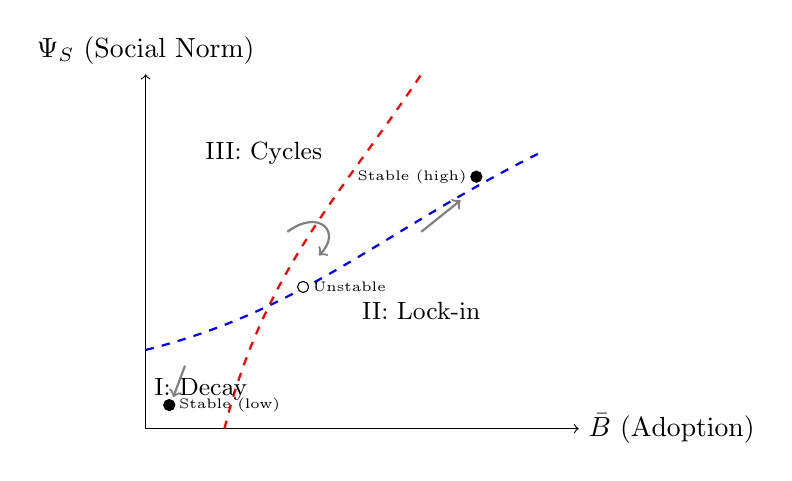
\begin{tikzpicture}[scale=1.0]
% Axes
\draw[->] (0,0) -- (5.5,0) node[right] {$\bar{B}$ (Adoption)};
\draw[->] (0,0) -- (0,4.5) node[above] {$\Psi_S$ (Social Norm)};

% Regime boundaries
\draw[thick, dashed, blue] (0,1) .. controls (2,1.5) and (3,2.5) .. (5,3.5);
\draw[thick, dashed, red] (1,0) .. controls (1.5,2) and (2.5,3) .. (3.5,4.5);

% Regime labels
\node at (0.7,0.5) {\small I: Decay};
\node at (3.5,1.5) {\small II: Lock-in};
\node at (1.5,3.5) {\small III: Cycles};

% Fixed points
\filldraw[black] (0.3,0.3) circle (2pt) node[right] {\tiny Stable (low)};
\filldraw[black] (4.2,3.2) circle (2pt) node[left] {\tiny Stable (high)};
\filldraw[white] (2,1.8) circle (2pt);
\draw (2,1.8) circle (2pt) node[right] {\tiny Unstable};

% Trajectories
\draw[->, thick, gray] (0.5,0.8) -- (0.35,0.4);
\draw[->, thick, gray] (3.5,2.5) -- (4,2.9);
\draw[->, thick, gray] (1.8,2.5) .. controls (2.2,2.8) and (2.5,2.5) .. (2.2,2.2);
\end{tikzpicture}
\end{center}

\textbf{Critical Mass Condition (Tipping Point):}
\begin{equation}
\bar{B}^* = \frac{\lambda_0 \cdot A^* + \mu_0 \cdot W^*}{\kappa_S + \kappa_T + \kappa_I}
\end{equation}

Once $\bar{B} > \bar{B}^*$, positive feedback dominates and behavior becomes self-sustaining.

\textbf{Empirical Validation:}
\begin{itemize}[nosep]
\item Regime I matches RCT decay observations (30--50\% pilot-to-scale) \citep{dellavigna2022rcts}
\item Regime II matches successful norm shifts (seatbelts, smoking decline) \citep{cialdini2004social}
\item Regime III matches fad dynamics (diet trends, exercise fads) \citep{rogers2003diffusion}
\end{itemize}

\end{tcolorbox}

\begin{tcolorbox}[colback=red!5!white, colframe=red!75!black,
    title=\textbf{Theorem NTM-T8: Optimal Intervention Timing Rule}]

\textbf{Statement:} Given UNTCM dynamics, the optimal intervention time $t^*$ maximizes the intervention's long-run impact:

\begin{equation}
t^* = \argmax_{t} \left[ \underbrace{\frac{\partial \bar{B}_\infty}{\partial I(t)}}_{\text{Marginal Impact}} \cdot \underbrace{\frac{1}{C(t)}}_{\text{Cost Efficiency}} \cdot \underbrace{P(\text{Regime II} | t)}_{\text{Lock-in Probability}} \right]
\label{eq:optimal-timing}
\end{equation}

\textbf{Intuition:} Intervene when:
\begin{enumerate}[nosep]
\item Marginal impact is high (system near tipping point)
\item Costs are low (favorable institutional context)
\item Lock-in probability is high (social norms supportive)
\end{enumerate}

\textbf{Practical Decision Rules:}

\begin{center}
\renewcommand{\arraystretch}{1.3}
\begin{tabular}{@{}lll@{}}
\toprule
\textbf{Context State} & \textbf{Optimal Timing} & \textbf{Intervention Type} \\
\midrule
$\Psi_S$ rising, $\bar{B}$ low & Wait for momentum & Light (AWARE, READY) to catalyze \\
$\Psi_S$ stable, $\bar{B}$ near $\bar{B}^*$ & Intervene NOW & Heavy (WHO, WHAT$_S$, WHAT$_F$) to tip \\
$\Psi_S$ falling, $\bar{B}$ high & Intervene to maintain & Identity (WHO) to lock in \\
$\Psi_E$ shock expected & Pre-position & Commitment (HOW) before shock \\
$\Psi_I$ changing & Wait for clarity & Hold until new equilibrium \\
\bottomrule
\end{tabular}
\end{center}

\textbf{Window of Opportunity:}

The intervention window $\Delta t_{opt}$ where timing matters most:
\begin{equation}
\Delta t_{opt} \approx \frac{1}{\max(\lambda, \mu, |\dot{\Psi}|)}
\end{equation}

For fast-changing contexts, the window is narrow. For stable contexts, timing is less critical.

\textbf{Connection to Portfolio Archetypes (Chapter 20):}
\begin{itemize}[nosep]
\item \textbf{Quick Wins:} Use when $\Delta t_{opt}$ is short (fast decay, urgent)
\item \textbf{Sustainable:} Use when targeting Regime II lock-in
\item \textbf{Low-Risk:} Use when $\Psi$ volatility is high (Regime III risk)
\end{itemize}

\end{tcolorbox}

\begin{tcolorbox}[colback=gray!5!white, colframe=gray!75!black,
    title=\textbf{UNTCM Parameter Summary Table}]

\begin{center}
\renewcommand{\arraystretch}{1.2}
\begin{tabular}{@{}llll@{}}
\toprule
\textbf{Parameter} & \textbf{Symbol} & \textbf{Typical Range} & \textbf{Source} \\
\midrule
\multicolumn{4}{l}{\textit{Baseline Decay Rates (context-neutral)}} \\
Awareness decay & $\lambda_0$ & 0.1--0.3/week & Ebbinghaus, Bordalo \\
Willingness decay & $\mu_0$ & 0.05--0.15/week & Laibson, Frederick \\
Threshold drift & $\delta_0$ & 0.01--0.05/month & O'Donoghue, Akerlof \\
\midrule
\multicolumn{4}{l}{\textit{Context Sensitivity (how much $\Psi$ affects decay)}} \\
Social norm sensitivity & $\alpha_S$ & 0.3--0.7 & Cialdini, Bicchieri \\
Technology sensitivity & $\alpha_T$ & 0.2--0.5 & Rogers \\
Economic sensitivity & $\alpha_E$ & 0.1--0.3 & Market calibration \\
Institutional sensitivity & $\alpha_I$ & 0.05--0.2 & North \\
Cultural sensitivity & $\alpha_C$ & 0.01--0.1 & Boyd \& Richerson \\
\midrule
\multicolumn{4}{l}{\textit{Feedback Strengths (how much behavior affects $\Psi$)}} \\
Social feedback & $\kappa_S$ & 0.3--0.5 & Granovetter thresholds \\
Technology feedback & $\kappa_T$ & 0.2--0.4 & Network effects \\
Institutional feedback & $\kappa_I$ & 0.05--0.15 & Policy feedback \\
\midrule
\multicolumn{4}{l}{\textit{Critical Thresholds}} \\
Tipping point & $\bar{B}^*$ & 10--25\% & Centola, Granovetter \\
Lock-in threshold & $\Psi_S^{lock}$ & 0.6--0.8 & Norm stability \\
\bottomrule
\end{tabular}
\end{center}

\textbf{Note:} All parameters require domain-specific calibration via Appendix UNMAPPED_BBB methods. Values shown are order-of-magnitude estimates from behavioral economics literature.

\end{tcolorbox}

%===============================================================================
% UNTCM METHODOLOGY
%===============================================================================

\section{UNTCM Methodology}
\label{sec:untcm-methodology}

This section provides the computational and statistical infrastructure for implementing, calibrating, and extending the UNTCM framework.

\begin{tcolorbox}[colback=blue!5!white, colframe=blue!75!black,
    title=\textbf{Method UNTCM-M1: Computational Implementation}]

\textbf{Discretization of the Coupled ODE System:}

The continuous UNTCM (\ref{eq:untcm-odes}) must be discretized for numerical simulation. Using Euler-Maruyama scheme with time step $\Delta t$:

\begin{equation}
\boxed{
\begin{aligned}
A_{t+1} &= A_t - \lambda(\vec{\Psi}_t) \cdot A_t \cdot \Delta t + I_A(t) \cdot \Delta t \\
W_{t+1} &= W_t - \mu(\vec{\Psi}_t) \cdot W_t \cdot \Delta t + I_W(t) \cdot \Delta t \\
\theta_{t+1} &= \theta_t + \delta(\vec{\Psi}_t) \cdot \Delta t + I_\theta(t) \cdot \Delta t \\
\Psi_{k,t+1} &= \Psi_{k,t} + \mu_k \cdot \Delta t + \kappa_k \cdot \bar{B}_t \cdot \Delta t + \sigma_k \sqrt{\Delta t} \cdot \epsilon_{k,t}
\end{aligned}
}
\label{eq:untcm-discrete}
\end{equation}

where $\epsilon_{k,t} \sim \mathcal{N}(0,1)$ i.i.d.

\textbf{Algorithm: UNTCM Simulation}

\begin{verbatim}
def simulate_untcm(params, T, dt, N_agents, interventions=None):
    """
    Simulate UNTCM dynamics for N agents over T time units.

    Parameters:
    - params: dict with lambda0, mu0, delta0, alpha_k, kappa_k, sigma_k
    - T: simulation horizon
    - dt: time step (recommend dt <= 0.01)
    - N_agents: number of agents (for aggregate behavior)
    - interventions: list of (t, type, intensity) tuples

    Returns:
    - trajectories: dict with A(t), W(t), theta(t), Psi(t), B_bar(t)
    """
    n_steps = int(T / dt)

    # Initialize state vectors
    A = np.zeros((n_steps, N_agents))
    W = np.zeros((n_steps, N_agents))
    theta = np.zeros((n_steps, N_agents))
    Psi = np.zeros((n_steps, 5))  # 5 context dimensions

    # Initial conditions (from calibration or BBB)
    A[0] = params['A0']
    W[0] = params['W0']
    theta[0] = params['theta0']
    Psi[0] = params['Psi0']

    for t in range(n_steps - 1):
        # Compute context-modulated decay rates
        lambda_t = compute_lambda(Psi[t], params)
        mu_t = compute_mu(Psi[t], params)
        delta_t = compute_delta(Psi[t], params)

        # Compute aggregate behavior
        B_bar = compute_adoption_rate(A[t], W[t], theta[t])

        # Get intervention inputs at time t
        I_A, I_W, I_theta = get_interventions(t, interventions)

        # Update individual states (vectorized)
        A[t+1] = A[t] * (1 - lambda_t * dt) + I_A * dt
        W[t+1] = W[t] * (1 - mu_t * dt) + I_W * dt
        theta[t+1] = theta[t] + delta_t * dt + I_theta * dt

        # Update context (with stochastic noise)
        noise = np.random.randn(5) * np.sqrt(dt)
        Psi[t+1] = Psi[t] + params['mu_psi'] * dt \
                   + params['kappa'] * B_bar * dt \
                   + params['sigma_psi'] * noise

    return {'A': A, 'W': W, 'theta': theta, 'Psi': Psi}
\end{verbatim}

\textbf{Numerical Stability:}
\begin{itemize}[nosep]
\item Time step: $\Delta t \leq \min(1/\lambda_{max}, 1/\mu_{max})$ for stability
\item Recommended: $\Delta t = 0.01$ (weekly time unit) or $\Delta t = 0.001$ (daily)
\item For stiff systems: Use implicit Euler or Runge-Kutta 4th order
\end{itemize}

\textbf{Computational Complexity:} $O(T \cdot N)$ per simulation run.

\end{tcolorbox}

\begin{tcolorbox}[colback=green!5!white, colframe=green!75!black,
    title=\textbf{Method UNTCM-M2: Parameter Calibration Protocol}]

\textbf{Challenge:} UNTCM has 15+ parameters. How to calibrate from data?

\textbf{Three-Stage Calibration Protocol:}

\begin{center}
\renewcommand{\arraystretch}{1.3}
\begin{tabular}{@{}clll@{}}
\toprule
\textbf{Stage} & \textbf{Parameters} & \textbf{Data Source} & \textbf{Method} \\
\midrule
1 & $\lambda_0, \mu_0, \delta_0$ & Literature meta-analysis & Appendix UNMAPPED_BBB lookup \\
2 & $\alpha_k, \beta_k, \gamma_k$ & Panel data with context variation & GMM / MLE \\
3 & $\kappa_k, \sigma_k$ & Time series of $\bar{B}(t)$ and $\Psi(t)$ & State-space estimation \\
\bottomrule
\end{tabular}
\end{center}

\textbf{Stage 1: Baseline Decay Rates (Literature-Based)}

Use Appendix UNMAPPED_BBB Parameter Repository:
\begin{equation}
\lambda_0 = \text{BBB.lookup}(\text{domain}, \text{``awareness\_decay''})
\end{equation}

Default values if domain-specific data unavailable:
\begin{itemize}[nosep]
\item Health behaviors: $\lambda_0 \approx 0.15$/week, $\mu_0 \approx 0.08$/week
\item Financial behaviors: $\lambda_0 \approx 0.20$/week, $\mu_0 \approx 0.12$/week
\item Environmental behaviors: $\lambda_0 \approx 0.10$/week, $\mu_0 \approx 0.06$/week
\end{itemize}

\textbf{Stage 2: Context Sensitivity (Econometric Estimation)}

Given panel data $\{A_{it}, W_{it}, \Psi_{kt}\}$, estimate via GMM:
\begin{equation}
\min_{\alpha} \sum_{i,t} \left( \Delta A_{it} + \lambda_0 \prod_k e^{-\alpha_k \Psi_{kt}} \cdot A_{it} \right)^2
\end{equation}

Identification requires sufficient context variation across time or cross-section.

\textbf{Stage 3: Feedback Parameters (State-Space Model)}

Cast UNTCM as state-space model:
\begin{align}
\text{State:} \quad & \mathbf{x}_t = (A_t, W_t, \theta_t, \Psi_{1t}, ..., \Psi_{5t})' \\
\text{Observation:} \quad & y_t = \bar{B}_t + \nu_t \\
\text{Transition:} \quad & \mathbf{x}_{t+1} = f(\mathbf{x}_t; \boldsymbol{\theta}) + \mathbf{w}_t
\end{align}

Estimate $\kappa_k, \sigma_k$ via:
\begin{itemize}[nosep]
\item Kalman Filter (linear approximation)
\item Particle Filter (full nonlinear)
\item MCMC (Bayesian with priors from literature)
\end{itemize}

\textbf{Validation Protocol:}
\begin{enumerate}[nosep]
\item Split data: 70\% calibration, 30\% validation
\item Out-of-sample prediction: Compare $\hat{\bar{B}}(t)$ to observed $\bar{B}(t)$
\item Regime classification accuracy: Does model correctly predict I/II/III?
\item Sensitivity analysis: Vary parameters $\pm 20\%$, check stability
\end{enumerate}

\textbf{Connection to LLMMC (Appendix UNMAPPED_LLM):}
When empirical data is sparse, use LLM Monte Carlo to generate synthetic parameter distributions based on behavioral economics literature.

\end{tcolorbox}

\begin{tcolorbox}[colback=purple!5!white, colframe=purple!75!black,
    title=\textbf{Method UNTCM-M3: Stochastic Extension (Full SDE)}]

\textbf{Motivation:} The basic UNTCM treats noise only in context dynamics. For full uncertainty quantification, extend to stochastic differential equations (SDEs) for all state variables.

\textbf{Full Stochastic UNTCM (Itô Form):}

\begin{equation}
\boxed{
\begin{aligned}
dA_t &= \left[ -\lambda(\vec{\Psi}_t) \cdot A_t + I_A(t) \right] dt + \sigma_A \cdot A_t \cdot dW_t^A \\
dW_t &= \left[ -\mu(\vec{\Psi}_t) \cdot W_t + I_W(t) \right] dt + \sigma_W \cdot W_t \cdot dW_t^W \\
d\theta_t &= \left[ \delta(\vec{\Psi}_t) + I_\theta(t) \right] dt + \sigma_\theta \cdot dW_t^\theta \\
d\Psi_{kt} &= \left[ \mu_k + \kappa_k \cdot \bar{B}_t \right] dt + \sigma_k \cdot dW_t^k
\end{aligned}
}
\label{eq:untcm-sde}
\end{equation}

where $W_t^A, W_t^W, W_t^\theta, W_t^k$ are independent Wiener processes.

\textbf{Interpretation of Noise Terms:}
\begin{itemize}[nosep]
\item $\sigma_A \cdot A_t \cdot dW^A$: Geometric Brownian motion for awareness (multiplicative noise, always positive)
\item $\sigma_W \cdot W_t \cdot dW^W$: Same for willingness
\item $\sigma_\theta \cdot dW^\theta$: Additive noise for threshold (can go negative = more permissive)
\item $\sigma_k \cdot dW^k$: Context shocks (already in basic model)
\end{itemize}

\textbf{Key Results from Stochastic Analysis:}

\textit{1. Probability of Regime Transition:}
\begin{equation}
P(\text{Regime I} \to \text{Regime II} | t) = \Phi\left( \frac{\bar{B}_t - \bar{B}^*}{\sigma_{eff} \sqrt{t}} \right)
\end{equation}
where $\sigma_{eff}^2 = \sigma_A^2 + \sigma_W^2 + \sum_k \kappa_k^2 \sigma_k^2$.

\textit{2. Expected First Passage Time to Tipping:}
\begin{equation}
\mathbb{E}[\tau^*] = \frac{2}{\sigma_{eff}^2} \int_{\bar{B}_0}^{\bar{B}^*} \frac{\bar{B}^* - x}{\mu_{drift}(x)} dx
\end{equation}

\textit{3. Variance of Long-Run Adoption:}
\begin{equation}
\text{Var}(\bar{B}_\infty) = \frac{\sum_k \sigma_k^2}{2 \cdot |\text{eigenvalue of stable fixed point}|}
\end{equation}

\textbf{Monte Carlo Confidence Intervals:}

For intervention planning, run $M$ simulation paths and compute:
\begin{itemize}[nosep]
\item Point estimate: $\hat{\bar{B}}(T) = \frac{1}{M} \sum_{m=1}^{M} \bar{B}^{(m)}(T)$
\item 95\% CI: $[\bar{B}_{0.025}(T), \bar{B}_{0.975}(T)]$ from empirical quantiles
\item Regime probabilities: $\hat{P}(\text{Regime II}) = \frac{1}{M} \sum_m \mathbb{1}\{\bar{B}^{(m)}(T) > \bar{B}^*\}$
\end{itemize}

\textbf{Recommended $M$:} $M \geq 1000$ for stable estimates, $M \geq 10000$ for tail probabilities.

\end{tcolorbox}

\begin{tcolorbox}[colback=red!5!white, colframe=red!75!black,
    title=\textbf{Method UNTCM-M4: Optimal Control Framework}]

\textbf{Problem:} Given limited intervention budget $B_{total}$, how to optimally allocate interventions $I_A(t), I_W(t), I_\theta(t)$ over time?

\textbf{Optimal Control Formulation:}

\begin{equation}
\max_{I_A, I_W, I_\theta} \int_0^T \underbrace{U(\bar{B}(t))}_{\text{Benefit}} - \underbrace{C(I_A, I_W, I_\theta)}_{\text{Cost}} \, dt
\label{eq:optimal-control}
\end{equation}

subject to UNTCM dynamics (\ref{eq:untcm-odes}) and budget constraint:
\begin{equation}
\int_0^T \left[ c_A \cdot I_A(t) + c_W \cdot I_W(t) + c_\theta \cdot I_\theta(t) \right] dt \leq B_{total}
\end{equation}

\textbf{Hamiltonian:}
\begin{equation}
\begin{aligned}
H = & \, U(\bar{B}) - C(I_A, I_W, I_\theta) \\
    & + p_A \left[ -\lambda(\Psi) A + I_A \right] \\
    & + p_W \left[ -\mu(\Psi) W + I_W \right] \\
    & + p_\theta \left[ \delta(\Psi) + I_\theta \right] \\
    & + \sum_k p_{\Psi_k} \left[ \mu_k + \kappa_k \bar{B} \right]
\end{aligned}
\end{equation}

\textbf{Pontryagin Conditions (Necessary for Optimality):}

\begin{align}
\frac{\partial H}{\partial I_A} &= 0 \Rightarrow p_A = \frac{\partial C}{\partial I_A} \\
\frac{\partial H}{\partial I_W} &= 0 \Rightarrow p_W = \frac{\partial C}{\partial I_W} \\
\dot{p}_A &= -\frac{\partial H}{\partial A} = p_A \lambda(\Psi) - \frac{\partial U}{\partial \bar{B}} \frac{\partial \bar{B}}{\partial A}
\end{align}

\textbf{Key Insights from Optimal Control:}

\textit{1. Bang-Bang Structure:}
With linear costs, optimal policy is often bang-bang:
\begin{equation}
I^*(t) = \begin{cases}
I_{max} & \text{if shadow price } p(t) > \text{threshold} \\
0 & \text{otherwise}
\end{cases}
\end{equation}

\textit{2. Intervention Timing:}
Optimal to concentrate interventions when:
\begin{itemize}[nosep]
\item System is near tipping point ($\bar{B} \approx \bar{B}^*$)
\item Context is favorable ($\Psi_S$ high)
\item Decay rates are temporarily low (seasonal effects)
\end{itemize}

\textit{3. Intervention Mix:}
Relative allocation depends on cost-effectiveness ratios:
\begin{equation}
\frac{I_A^*}{I_W^*} = \frac{c_W}{c_A} \cdot \frac{\partial \bar{B}/\partial A}{\partial \bar{B}/\partial W}
\end{equation}

\textbf{Numerical Solution:}

\begin{verbatim}
def solve_optimal_control(params, T, B_total, method='shooting'):
    """
    Solve UNTCM optimal control problem.

    Methods:
    - 'shooting': Boundary value problem solver
    - 'collocation': Direct collocation
    - 'dp': Dynamic programming (discretized)
    - 'mpc': Model predictive control (rolling horizon)
    """
    if method == 'shooting':
        # Solve costate equations backward, state forward
        return scipy.integrate.solve_bvp(...)
    elif method == 'mpc':
        # Rolling horizon with re-optimization
        for t in range(0, T, horizon):
            I_opt = solve_finite_horizon(t, t+horizon)
            apply_intervention(I_opt[0])
            observe_state()
\end{verbatim}

\textbf{Connection to Portfolio Archetypes:}

| Archetype | Optimal Control Interpretation |
|-----------|-------------------------------|
| Quick Wins | High $I$ early, then zero |
| Sustainable | Moderate $I$ sustained to reach lock-in |
| Budget-Constrained | Sparse interventions at optimal timing |
| Low-Risk | Conservative $I$ with safety margin |

\end{tcolorbox}

%-------------------------------------------------------------------------------
% METHOD M5: Maintenance Cost Analysis
%-------------------------------------------------------------------------------

\begin{tcolorbox}[colback=orange!5!white, colframe=orange!75!black,
    title=\textbf{Method UNTCM-M5: Maintenance Cost Analysis}]

\textbf{Motivation:} From UNTCM-X5 (Status-Quo Lock-in), we know that maintaining the status quo becomes increasingly costly over time due to reference point drift and loss aversion amplification. M5 formalizes the intervention intensity required to maintain utility levels across FEPSDE dimensions at different time horizons.

\textbf{The Maintenance Paradox:} Status quo maintenance is NOT free. Natural decay requires continuous compensatory intervention, and the required intensity \emph{increases} over time due to X5.

\textbf{Cross-Reference Box:}
\begin{itemize}[nosep]
\item \textbf{Chapter 17 (Emergent Intervention Theory):} Emergent 10C intervention vectors used for maintenance
\item \textbf{Chapter 18 (Journey Integration):} Phase-specific maintenance requirements
\item \textbf{Chapter 19 (Segment Heterogeneity):} Segment-specific $\lambda_d^{(s)}$ decay rates
\item \textbf{Chapter 20 (Portfolio Archetypes):} ``Sustainable'' archetype for long-term maintenance
\end{itemize}

\textbf{FEPSDE-Specific Decay Rates:}

Each utility dimension $d \in \{\text{F, E, P, S, D, Ex}\}$ has a characteristic decay rate:

\begin{center}
\renewcommand{\arraystretch}{1.2}
\begin{tabular}{@{}clccl@{}}
\toprule
\textbf{Dim} & \textbf{Name} & \textbf{$\lambda_d$} & \textbf{Half-Life} & \textbf{Driver} \\
\midrule
F & Financial & 0.02/wk & 35 weeks & Budget constraints, inflation \\
E & Emotional & 0.15/wk & 4.6 weeks & Hedonic adaptation \\
P & Physical & 0.08/wk & 8.7 weeks & Habit decay, entropy \\
S & Social & 0.04/wk & 17 weeks & Relationship maintenance \\
D & Developmental & 0.01/wk & 69 weeks & Skill atrophy, obsolescence \\
Ex & Experiential & 0.20/wk & 3.5 weeks & Memory decay, novelty bias \\
\bottomrule
\end{tabular}
\end{center}

\textbf{Maintenance Cost Function:}

The intervention intensity $I_d(t)$ required to maintain utility level $U_d(0)$ in dimension $d$:

\begin{equation}
I_d^{maintain}(t) = \underbrace{\lambda_d \cdot U_d(0)}_{\text{Base decay compensation}} + \underbrace{\lambda_{LA} \cdot \eta_r \cdot (1 - e^{-\eta_r t}) \cdot \Delta\theta_d}_{\text{X5 loss aversion premium}}
\label{eq:maintenance-cost}
\end{equation}

where the second term captures the increasing ``stickiness'' of the status quo over time.

\textbf{Time Horizon Taxonomy:}

\begin{center}
\renewcommand{\arraystretch}{1.3}
\begin{tabular}{@{}lccl@{}}
\toprule
\textbf{Horizon} & \textbf{Duration} & \textbf{X5 Premium} & \textbf{Primary Intervention Types} \\
\midrule
Instant & $<$ 1 day & $\approx 0$ & AWARE, WHEN (Contextual) \\
Short & 1-4 weeks & $0.1-0.3\times$ & READY (Feedback), STAGE (Temporal) \\
Medium & 1-6 months & $0.5-1.0\times$ & WHO (Identity), WHAT$_S$ (Social) \\
Long & $>$ 6 months & $1.5-2.25\times$ & HOW (Commitment) + Portfolio \\
\bottomrule
\end{tabular}
\end{center}

\textbf{Three Utility Levels:}

Maintenance requirements differ by utility level (cf.\ Appendix UNMAPPED_AAA):

\begin{center}
\renewcommand{\arraystretch}{1.3}
\begin{tabular}{@{}lll@{}}
\toprule
\textbf{Level} & \textbf{Maintenance Mechanism} & \textbf{Key Intervention} \\
\midrule
$u_I$ (Individual) & Self-regulation, habits & READY (Feedback), WHEN (Defaults) \\
$u_C$ (Collective) & Social norms, reciprocity & WHAT$_S$ (Social), AWARE (Norms) \\
$u_D$ (Identity) & Value reinforcement & WHO (Identity), HOW (Commitment) \\
\bottomrule
\end{tabular}
\end{center}

\textbf{FEPSDE $\times$ Time Horizon Matrix:}

Required intervention intensity $I_d^{maintain}$ (scale: 1=minimal, 5=intensive):

\begin{center}
\renewcommand{\arraystretch}{1.2}
\begin{tabular}{@{}lcccc@{}}
\toprule
\textbf{Dimension} & \textbf{Instant} & \textbf{Short} & \textbf{Medium} & \textbf{Long} \\
\midrule
Financial (F) & 1 & 1 & 2 & 3 \\
Emotional (E) & 2 & 3 & 4 & 5 \\
Physical (P) & 1 & 2 & 3 & 4 \\
Social (S) & 1 & 2 & 2 & 3 \\
Developmental (D) & 1 & 1 & 2 & 2 \\
Experiential (Ex) & 2 & 4 & 5 & 5 \\
\bottomrule
\end{tabular}
\end{center}

\textbf{Key Insight:} Emotional (E) and Experiential (Ex) dimensions have the highest maintenance costs due to fast decay ($\lambda_E, \lambda_{Ex}$ high) and strong hedonic adaptation. Physical (P) and Social (S) require moderate maintenance. Financial (F) and Developmental (D) are most ``durable'' but still decay.

\textbf{Theorem M5-T1: Maintenance Cost Superlinearity}

Under X5 (Loss Aversion Lock-in), the cumulative maintenance cost grows \emph{superlinearly} with time:

\begin{equation}
C_{maintain}(T) = \int_0^T I_d^{maintain}(t) \, dt = \lambda_d U_d(0) T + \lambda_{LA} \Delta\theta_d \left[ T - \frac{1 - e^{-\eta_r T}}{\eta_r} \right]
\label{eq:cumulative-maintenance}
\end{equation}

\textbf{Corollary:} For long horizons ($T \gg 1/\eta_r$):
\begin{equation}
C_{maintain}(T) \approx (\lambda_d U_d(0) + \lambda_{LA} \Delta\theta_d) \cdot T - \frac{\lambda_{LA} \Delta\theta_d}{\eta_r}
\end{equation}

The asymptotic maintenance rate is $(1 + \lambda_{LA})$ times the base decay rate---a 225\% premium.

\textbf{Policy Implication (→ Chapter 17, Chapter 20):}

\begin{itemize}[nosep]
\item \textbf{Quick Wins archetype:} Addresses immediate maintenance (instant/short)
\item \textbf{Sustainable archetype:} Explicitly budgets for long-term maintenance costs
\item \textbf{Portfolio design:} Include WHO (Identity) and HOW (Commitment) for maintenance efficiency
\item \textbf{Phase-specific (→ Chapter 18):} Maintenance in Phase 5 (Stable) requires ongoing WHAT$_S$ (Social norms)
\item \textbf{Segment-specific (→ Chapter 19):} High-decay segments ($\beta < 1$ present-biased) need more frequent maintenance
\end{itemize}

\textbf{Reference Point Reset Strategy:}

To reduce maintenance costs, periodically reset the reference point using Fresh Start Effect (cf.\ X5):
\begin{equation}
C_{maintain}^{reset}(T) < C_{maintain}(T) \quad \text{if resets at } t_1, t_2, ... \text{ with } t_{k+1} - t_k < 2/\eta_r
\end{equation}

\textbf{Worked Example: Corporate Wellness Program}

A company wants to maintain employee engagement in a wellness program over 12 months.

\begin{center}
\renewcommand{\arraystretch}{1.2}
\begin{tabular}{@{}lcccl@{}}
\toprule
\textbf{Month} & \textbf{Phase} & \textbf{$I_{maintain}$} & \textbf{Cost Index} & \textbf{Interventions} \\
\midrule
1 & Launch & 1.0 & 1.0 & AWARE (Kickoff), WHEN (Defaults) \\
3 & Short & 1.5 & 1.5 & READY (Progress feedback) \\
6 & Medium & 2.2 & 2.2 & WHAT$_S$ (Team challenges), WHO (Identity badges) \\
9 & Long & 2.8 & 2.8 & HOW (Annual commitment renewal) \\
12 & Annual & 3.2 & 3.2 & Fresh Start (New Year reset) \\
\midrule
\multicolumn{2}{@{}l}{\textbf{Cumulative}} & --- & \textbf{10.7} & \textbf{vs.\ 5.0 (naive linear estimate)} \\
\bottomrule
\end{tabular}
\end{center}

\textbf{Insight:} The naive estimate ($5.0 = 1.0 \times 5$ intervals) underestimates true maintenance costs by 114\% due to X5 premium.

\textbf{Definition M5-D1: Minimal Maintenance Portfolio}

The \textbf{Minimal Maintenance Portfolio} $\mathcal{P}_{maintain}^{min}(H)$ for time horizon $H$ is the smallest set of emergent intervention vectors that maintains all FEPSDE dimensions above threshold and preserves all three utility levels ($u_I$, $u_C$, $u_D$):

\begin{equation}
\mathcal{P}_{maintain}^{min}(H) = \arg\min_{P \subseteq \mathcal{I}} |P| \quad \text{s.t.} \quad \forall d \in \text{FEPSDE}: U_d(H) \geq U_d(0) - \epsilon
\end{equation}
where $\mathcal{I}$ is the set of feasible intervention vectors in $[0,1]^9$.

\textbf{Theorem M5-T2: Horizon-Dependent Portfolio Cardinality}

The minimal portfolio size grows with time horizon:

\begin{equation}
|\mathcal{P}_{maintain}^{min}(H)| = \begin{cases}
3 & H < 1 \text{ day (Instant)} \\
5 & H \in [1\text{d}, 4\text{w}] \text{ (Short)} \\
5 & H \in [4\text{w}, 6\text{m}] \text{ (Medium)} \\
6 & H > 6\text{m} \text{ (Long)}
\end{cases}
\end{equation}

\textbf{Minimal Portfolio Specification by Horizon:}

\begin{center}
\renewcommand{\arraystretch}{1.3}
\begin{tabular}{@{}lccccccccc@{}}
\toprule
\textbf{Horizon} & AWA & RDY & WHN & STG & WHO & W$_S$ & W$_F$ & HOW & $|\mathcal{P}^{min}|$ \\
\midrule
Instant & $\bullet$ & & & & $\bullet$ & $\bullet$ & & & 3 \\
Short & $\bullet$ & $\bullet$ & $\bullet$ & & & $\bullet$ & & $\bullet$ & 5 \\
Medium & $\bullet$ & & & $\bullet$ & $\bullet$ & $\bullet$ & $\bullet$ & & 5 \\
Long & $\bullet$ & & & $\bullet$ & $\bullet$ & $\bullet$ & $\bullet$ & $\bullet$ & 6 \\
\bottomrule
\end{tabular}
\end{center}

\textbf{Utility Level → Intervention Type Mapping:}

\begin{center}
\renewcommand{\arraystretch}{1.2}
\begin{tabular}{@{}lll@{}}
\toprule
\textbf{Utility Level} & \textbf{Primary Interventions} & \textbf{Mechanism} \\
\midrule
$u_I$ (Individual) & READY (Feedback), WHEN (Context), WHAT$_F$ (Financial) & Self-regulation, habits \\
$u_C$ (Collective) & AWARE, WHAT$_S$ (Social) & Social norms, reciprocity \\
$u_D$ (Identity) & WHO (Identity), HOW (Commitment) & Value reinforcement \\
\bottomrule
\end{tabular}
\end{center}

\textbf{Key Findings (M5-T2):}
\begin{itemize}[nosep]
\item \textbf{T1 (Awareness) + T6 (Social)} are backbone interventions---required at ALL horizons
\item \textbf{T5 (Identity)} becomes critical from medium-term---status quo threatens value alignment
\item \textbf{T7 (Financial)} only needed medium+ when X5 premium demands stronger incentives
\item \textbf{T8 (Commitment)} needed at short (reminder) and long (renewal) horizons
\item \textbf{Instant portfolio} (3 interventions) can prevent immediate decay at minimal cost
\item \textbf{Long-term portfolio} (6 interventions) requires full toolkit due to X5 premium
\end{itemize}

\vspace{1em}
\hrule
\vspace{1em}

\textbf{Definition M5-D2: Portfolio Archetypes for Maintenance}

Beyond the minimal portfolio, we define five archetypes that span the Pareto-frontier between cost and effectiveness:

\begin{enumerate}[nosep]
\item \textbf{Minimal Portfolio} $\mathcal{P}^{min}(H)$: Smallest $|\mathcal{P}|$ satisfying maintenance constraint
\[
\mathcal{P}^{min}(H) = \arg\min_{\mathcal{P} \subseteq \{T1,...,T8\}} |\mathcal{P}| \quad \text{s.t.} \quad \forall d \in \text{FEPSDE}: U_d(H) \geq U_d(0) - \epsilon
\]

\item \textbf{Cost-Optimal Portfolio} $\mathcal{P}^{cost}(H)$: Minimize total cost
\[
\mathcal{P}^{cost}(H) = \arg\min_{\mathcal{P}} \sum_{T_i \in \mathcal{P}} c_i(H) \cdot (1 + \xi_{X5}(H)) \quad \text{s.t. maintenance constraint}
\]
where $\xi_{X5}(H)$ is the X5 loss aversion premium for horizon $H$.

\item \textbf{Effectiveness-Optimal Portfolio} $\mathcal{P}^{eff}(H)$: Maximize effectiveness per unit cost
\[
\mathcal{P}^{eff}(H) = \arg\max_{\mathcal{P}} \frac{\sum_{T_i \in \mathcal{P}} \Delta P_{eff,i}}{\sum_{T_i \in \mathcal{P}} c_i(H)}
\]

\item \textbf{Risk-Adjusted Portfolio} $\mathcal{P}^{risk}(H)$: Minimize maintenance failure variance
\[
\mathcal{P}^{risk}(H) = \arg\min_{\mathcal{P}} \text{Var}\left[\min_d U_d(H) | \mathcal{P}\right] \quad \text{s.t.} \quad \mathbb{E}\left[\min_d U_d(H)\right] \geq U_d(0) - \epsilon
\]

\item \textbf{Segment-Specific Portfolio} $\mathcal{P}^{seg}(H, s)$: Apply segment multipliers $\sigma_{s,i}$ from I4
\[
\mathcal{P}^{seg}(H, s) = \arg\max_{\mathcal{P}} \sum_{T_i \in \mathcal{P}} \sigma_{s,i} \cdot \text{eff}_i(H) - \lambda \cdot \text{Cost}(\mathcal{P})
\]
where $\sigma_{s,i}$ is the segment $s$ multiplier for intervention type $T_i$ (see Chapter 19).
\end{enumerate}

\vspace{0.5em}

\textbf{Theorem M5-T3: Maintenance Portfolio Pareto-Frontier}

For any time horizon $H$, the set of Pareto-efficient portfolios forms a frontier $\mathcal{F}(H)$:

\[
\mathcal{F}(H) = \left\{ \mathcal{P} : \nexists \mathcal{P}' \text{ with } \text{Cost}(\mathcal{P}') \leq \text{Cost}(\mathcal{P}) \text{ and } \text{Eff}(\mathcal{P}') \geq \text{Eff}(\mathcal{P}) \right\}
\]

\textbf{Properties of $\mathcal{F}(H)$:}
\begin{enumerate}[nosep]
\item $\mathcal{P}^{min}(H), \mathcal{P}^{cost}(H) \in \mathcal{F}(H)$ (both are Pareto-efficient)
\item $|\mathcal{F}(H)|$ is non-decreasing in $H$ (more options for longer horizons)
\item The frontier shifts outward with X5 premium: $\text{Cost}(\mathcal{F}(H_2)) > \text{Cost}(\mathcal{F}(H_1))$ for $H_2 > H_1$
\item Segment-specific portfolios may dominate general portfolios: $\mathcal{P}^{seg} \succ \mathcal{P}^{min}$ when $\sigma_{s,i} > 1.3$
\end{enumerate}

\textbf{Portfolio Selection Rule:}
\begin{center}
\renewcommand{\arraystretch}{1.2}
\begin{tabular}{@{}ll@{}}
\toprule
\textbf{Constraint} & \textbf{Select} \\
\midrule
Budget-constrained & $\mathcal{P}^{cost}(H)$ \\
Risk-averse stakeholder & $\mathcal{P}^{risk}(H)$ \\
Maximizing ROI & $\mathcal{P}^{eff}(H)$ \\
Unknown segment & $\mathcal{P}^{min}(H)$ \\
Known high-multiplier segment & $\mathcal{P}^{seg}(H, s)$ \\
\bottomrule
\end{tabular}
\end{center}

\vspace{0.5em}
\hrule
\vspace{0.5em}

\textbf{Connection to Chapter 16:} Worked example (Anna's heat pump) demonstrates full 12-month maintenance schedule and portfolio selection.

\textbf{Connection to Chapter 20:} The ``Sustainable'' archetype explicitly budgets for $\mathcal{P}_{maintain}^{min}(\text{Long})$ or higher.

\end{tcolorbox}

\begin{tcolorbox}[colback=yellow!5!white, colframe=yellow!75!black,
    title=\textbf{UNTCM Methodology: Quick Reference}]

\begin{center}
\renewcommand{\arraystretch}{1.3}
\begin{tabular}{@{}llll@{}}
\toprule
\textbf{Method} & \textbf{Purpose} & \textbf{Input} & \textbf{Output} \\
\midrule
M1 (Computational) & Simulate trajectories & Parameters, $T$, $N$ & $A(t), W(t), \Psi(t)$ \\
M2 (Calibration) & Estimate parameters & Panel/time-series data & $\hat{\lambda}, \hat{\kappa}, \hat{\sigma}$ \\
M3 (Stochastic) & Uncertainty quantification & Noise parameters & Confidence intervals \\
M4 (Optimal Control) & Intervention planning & Budget, costs & $I^*(t)$ schedule \\
M5 (Maintenance) & Status quo preservation & $\lambda_d$, horizon, X5 & $I^{maintain}(t)$ schedule \\
\bottomrule
\end{tabular}
\end{center}

\textbf{Typical Workflow:}
\begin{enumerate}[nosep]
\item \textbf{Calibrate} (M2): Use historical data + BBB to estimate parameters
\item \textbf{Simulate} (M1): Run baseline trajectory (no intervention)
\item \textbf{Quantify Uncertainty} (M3): Monte Carlo for confidence intervals
\item \textbf{Optimize} (M4): Find best intervention schedule given budget
\item \textbf{Validate}: Compare predicted vs. actual outcomes (feedback to M2)
\end{enumerate}

\textbf{Software Requirements:}
\begin{itemize}[nosep]
\item Python: numpy, scipy, pymc3 (Bayesian), casadi (optimal control)
\item R: deSolve, pomp (state-space), optimx
\item Julia: DifferentialEquations.jl, Turing.jl, JuMP.jl
\end{itemize}

\end{tcolorbox}

%===============================================================================
% UNTCM FRAMEWORK INTEGRATION
%===============================================================================

\section{UNTCM Framework Integration}
\label{sec:untcm-integration}

This section connects UNTCM to the core EBF components: BCJ (Journey Phases), Emergent 10C Intervention Vectors, FEPSDE (Utility Dimensions), and Segments.

\begin{tcolorbox}[colback=blue!5!white, colframe=blue!75!black,
    title=\textbf{Integration UNTCM-I1: BCJ Journey Phase Mapping}]

\textbf{Connection to Appendix UNMAPPED_AW (CORE-STAGE):}

The Behavioral Change Journey (BCJ) defines 5 phases $\phi \in \{1, 2, 3, 4, 5\}$. UNTCM regimes map naturally onto journey progression:

\begin{center}
\renewcommand{\arraystretch}{1.3}
\begin{tabular}{@{}cllll@{}}
\toprule
\textbf{Phase} & \textbf{Name} & \textbf{UNTCM State} & \textbf{Regime} & \textbf{Dynamics} \\
\midrule
$\phi = 1$ & Pre-contemplation & $A \approx 0$, $W$ low & I (Decay) & Stable low equilibrium \\
$\phi = 2$ & Contemplation & $A$ rising, $W$ low & I → II transition & Near tipping point \\
$\phi = 3$ & Preparation & $A$ high, $W$ rising & II (Feedback) & Positive momentum \\
$\phi = 4$ & Action & $A, W$ high, $\bar{B}$ rising & II (Lock-in) & Self-sustaining \\
$\phi = 5$ & Maintenance & $\bar{B} > \bar{B}^*$, $\Psi_S$ high & II (Stable high) & Identity crystallized \\
\bottomrule
\end{tabular}
\end{center}

\textbf{Phase Transition as Regime Change:}

Journey phase transitions correspond to UNTCM regime transitions:
\begin{equation}
\phi_{t+1} = \phi_t + \mathbb{1}\{\text{Regime}_{t+1} \neq \text{Regime}_t\}
\end{equation}

\textbf{Key Insight:} Phase $\phi = 2 \to 3$ (Contemplation → Preparation) is the critical transition where the system moves from Regime I to Regime II. This is where interventions have maximum leverage.

\textbf{Phase-Specific UNTCM Parameters:}

\begin{center}
\renewcommand{\arraystretch}{1.2}
\begin{tabular}{@{}clll@{}}
\toprule
\textbf{Phase} & \textbf{$\lambda$ (Awareness Decay)} & \textbf{$\mu$ (Willingness Decay)} & \textbf{$\kappa$ (Feedback)} \\
\midrule
$\phi = 1$ & High (0.3/wk) & N/A (W ≈ 0) & Low (0.1) \\
$\phi = 2$ & Medium (0.2/wk) & High (0.15/wk) & Medium (0.3) \\
$\phi = 3$ & Low (0.1/wk) & Medium (0.10/wk) & High (0.5) \\
$\phi = 4$ & Very low (0.05/wk) & Low (0.05/wk) & Very high (0.7) \\
$\phi = 5$ & Minimal (0.02/wk) & Minimal (0.02/wk) & Saturated \\
\bottomrule
\end{tabular}
\end{center}

\textbf{Implication:} Decay rates decrease as journey progresses (habit formation, identity lock-in).

\end{tcolorbox}

\begin{tcolorbox}[colback=green!5!white, colframe=green!75!black,
    title=\textbf{Integration UNTCM-I2: 10C Intervention Vector Mapping}]

\textbf{Connection to Chapter 17 (Emergent Intervention Theory):}

Each emergent intervention vector (from the continuous $[0,1]^9$ space) acts on specific UNTCM state variables:

\begin{center}
\renewcommand{\arraystretch}{1.3}
\begin{tabular}{@{}clccccl@{}}
\toprule
\textbf{Type} & \textbf{Name} & \textbf{$I_A$} & \textbf{$I_W$} & \textbf{$I_\theta$} & \textbf{$\Delta\Psi$} & \textbf{Mechanism} \\
\midrule
T1 & Awareness & \checkmark\checkmark & & & & Direct $A$ boost \\
T2 & Feedback & \checkmark & \checkmark & $\downarrow$ & & Reduces threshold via learning \\
T3 & Contextual & & & $\downarrow\downarrow$ & $\Psi_T \uparrow$ & Choice architecture \\
T4 & Temporal & \checkmark & & $\downarrow$ & & Urgency, deadlines \\
T5 & Identity & & \checkmark\checkmark & & $\Psi_C \uparrow$ & Direct $W$ boost (intrinsic) \\
T6 & Social & \checkmark & \checkmark & & $\Psi_S \uparrow$ & Norm activation \\
T7 & Financial & & \checkmark\checkmark & $\downarrow$ & $\Psi_E$ & Extrinsic motivation \\
T8 & Commitment & & \checkmark & $\downarrow\downarrow$ & & Pre-commitment device \\
\bottomrule
\end{tabular}
\end{center}

\textbf{Legend:} \checkmark = moderate effect, \checkmark\checkmark = strong effect, $\downarrow$ = decrease, $\uparrow$ = increase

\textbf{UNTCM Intervention Input Functions:}

\begin{align}
I_A(t) &= \sum_{j \in \{1,2,4,6\}} \alpha_j \cdot T_j(t) \label{eq:I_A} \\
I_W(t) &= \sum_{j \in \{2,5,6,7,8\}} \beta_j \cdot T_j(t) \label{eq:I_W} \\
I_\theta(t) &= -\sum_{j \in \{2,3,4,7,8\}} \gamma_j \cdot T_j(t) \label{eq:I_theta}
\end{align}

where $T_j(t) \in [0, 1]$ is the intensity of intervention type $j$ at time $t$.

\textbf{Type-Specific Effectiveness Coefficients:}

\begin{center}
\renewcommand{\arraystretch}{1.2}
\begin{tabular}{@{}clllll@{}}
\toprule
\textbf{Type} & $\alpha_j$ (→ $A$) & $\beta_j$ (→ $W$) & $\gamma_j$ (→ $\theta$) & \textbf{Duration} & \textbf{Source} \\
\midrule
T1 & 0.3--0.5 & -- & -- & Days & Bordalo (2012) \\
T2 & 0.1--0.2 & 0.1--0.2 & 0.05--0.1 & Weeks & Feedback loops \\
T3 & -- & -- & 0.2--0.4 & Persistent & Thaler (2008) \\
T4 & 0.2--0.3 & -- & 0.1--0.2 & Days & Urgency effects \\
T5 & -- & 0.3--0.5 & -- & Months & Akerlof (2000) \\
T6 & 0.1--0.2 & 0.2--0.3 & -- & Weeks & Cialdini (2004) \\
T7 & -- & 0.2--0.4 & 0.1--0.3 & Variable & Gneezy (2011) \\
T8 & -- & 0.1--0.2 & 0.2--0.4 & Months & Commitment lit. \\
\bottomrule
\end{tabular}
\end{center}

\textbf{Crowding-Out in UNTCM Terms:}

T6 + T7 crowding: When both social ($\Psi_S \uparrow$) and financial ($\Psi_E$) are active:
\begin{equation}
\Delta W_{eff} = \beta_6 \cdot T_6 + \beta_7 \cdot T_7 + \underbrace{\gamma_{67} \cdot T_6 \cdot T_7}_{\text{Crowding (negative)}}
\end{equation}

where $\gamma_{67} \approx -0.2$ from Gneezy \& Rustichini (2000).

\end{tcolorbox}

\begin{tcolorbox}[colback=purple!5!white, colframe=purple!75!black,
    title=\textbf{Integration UNTCM-I3: FEPSDE Utility Decomposition}]

\textbf{Connection to Appendix UNMAPPED_C (CORE-WHAT):}

Willingness $W$ in UNTCM is not scalar but decomposes along FEPSDE utility dimensions:

\begin{equation}
\boxed{
W = \sum_{d \in \text{FEPSDE}} w_d \cdot W_d = w_F W_F + w_E W_E + w_P W_P + w_S W_S + w_D W_D + w_X W_X
}
\label{eq:W-fepsde}
\end{equation}

where:
\begin{itemize}[nosep]
\item $W_F$ = Financial willingness (monetary utility)
\item $W_E$ = Emotional willingness (hedonic utility)
\item $W_P$ = Procedural willingness (effort/hassle costs)
\item $W_S$ = Social willingness (norm alignment)
\item $W_D$ = Developmental willingness (growth/learning)
\item $W_X$ = eXternal willingness (environmental/ethical)
\end{itemize}

\textbf{Dimension-Specific Decay Rates:}

Each dimension has its own decay rate $\mu_d$:

\begin{center}
\renewcommand{\arraystretch}{1.2}
\begin{tabular}{@{}cllll@{}}
\toprule
\textbf{Dim} & \textbf{Name} & \textbf{$\mu_d$ (/week)} & \textbf{Decay Driver} & \textbf{Sustaining Factor} \\
\midrule
F & Financial & 0.05--0.10 & Habituation to reward & Increasing stakes \\
E & Emotional & 0.15--0.25 & Hedonic adaptation & Variety, novelty \\
P & Procedural & 0.02--0.05 & Habit formation & Simplification \\
S & Social & 0.10--0.15 & Norm salience decay & Social reinforcement \\
D & Developmental & 0.03--0.08 & Mastery plateau & New challenges \\
X & External & 0.05--0.12 & Value salience decay & Impact feedback \\
\bottomrule
\end{tabular}
\end{center}

\textbf{Vectorized UNTCM:}

The full UNTCM with FEPSDE decomposition:
\begin{equation}
\frac{d\vec{W}}{dt} = -\text{diag}(\vec{\mu}(\Psi)) \cdot \vec{W} + \vec{I}_W(t)
\end{equation}

where $\vec{W} = (W_F, W_E, W_P, W_S, W_D, W_X)'$ and $\vec{\mu} = (\mu_F, ..., \mu_X)'$.

\textbf{Emergent Intervention Vector to FEPSDE Mapping:}

\begin{center}
\renewcommand{\arraystretch}{1.2}
\begin{tabular}{@{}ccccccc@{}}
\toprule
\textbf{Type} & $W_F$ & $W_E$ & $W_P$ & $W_S$ & $W_D$ & $W_X$ \\
\midrule
T5 (Identity) & & & & \checkmark & \checkmark & \checkmark \\
T6 (Social) & & & & \checkmark\checkmark & & \\
T7 (Financial) & \checkmark\checkmark & & & & & \\
T8 (Commitment) & & & \checkmark & & \checkmark & \\
\bottomrule
\end{tabular}
\end{center}

\textbf{Implication:} Different intervention types target different $W$ components. Sustainable change requires multiple $W_d$ activated.

\end{tcolorbox}

\begin{tcolorbox}[colback=red!5!white, colframe=red!75!black,
    title=\textbf{Integration UNTCM-I4: Segment Heterogeneity}]

\textbf{Connection to Chapter 19 (Segmentation):}

Different segments $s \in S$ have heterogeneous UNTCM parameters:

\begin{equation}
\boxed{
\text{UNTCM}_s: \quad \lambda_s(\Psi), \quad \mu_s(\Psi), \quad \delta_s(\Psi), \quad \kappa_s
}
\label{eq:untcm-segment}
\end{equation}

\textbf{Segment-Specific Parameter Profiles:}

\begin{center}
\renewcommand{\arraystretch}{1.3}
\begin{tabular}{@{}lccccl@{}}
\toprule
\textbf{Segment} & $\lambda_s$ & $\mu_s$ & $\delta_s$ & $\kappa_s$ & \textbf{Archetype} \\
\midrule
Early Adopters & Low & Low & Low & High & Quick lock-in \\
Early Majority & Medium & Medium & Medium & Medium & Standard trajectory \\
Late Majority & High & High & High & Low & Slow conversion \\
Laggards & Very high & Very high & Very high & Very low & Resistant \\
\midrule
Loss Averse & Medium & High & High & Medium & Financial focus \\
Social Oriented & Low & Low & Low & Very high & Norm-driven \\
Autonomy Seeking & High & Medium & High & Low & Reactance risk \\
Present Biased & Very high & High & Very high & Medium & Immediate decay \\
\bottomrule
\end{tabular}
\end{center}

\textbf{Segment-Weighted Aggregate Dynamics:}

Population-level behavior is segment-weighted:
\begin{equation}
\bar{B}(t) = \sum_{s \in S} \pi_s \cdot \bar{B}_s(t)
\end{equation}

where $\pi_s$ is segment proportion and $\bar{B}_s(t)$ is segment-specific adoption.

\textbf{Heterogeneous Tipping Points:}

Each segment has its own tipping point $\bar{B}_s^*$:
\begin{equation}
\bar{B}_s^* = \frac{\lambda_{s,0} + \mu_{s,0}}{\kappa_s}
\end{equation}

\textbf{Strategic Implication:} Target segments with low $\bar{B}_s^*$ first (Early Adopters, Social Oriented) to build momentum, then cascade to higher-threshold segments.

\textbf{Segment Transition Dynamics:}

Success in segment $s$ affects other segments via $\kappa$:
\begin{equation}
\frac{d\Psi_S}{dt} = \sum_{s} \kappa_s \cdot \pi_s \cdot \bar{B}_s(t)
\end{equation}

High-$\kappa$ segments (Social Oriented) have outsized impact on norm evolution.

\end{tcolorbox}

\begin{tcolorbox}[colback=yellow!5!white, colframe=yellow!75!black,
    title=\textbf{UNTCM Framework Integration: Summary}]

\begin{center}
\renewcommand{\arraystretch}{1.3}
\begin{tabular}{@{}llll@{}}
\toprule
\textbf{Integration} & \textbf{EBF Component} & \textbf{UNTCM Mapping} & \textbf{Key Insight} \\
\midrule
I1 & BCJ (Journey) & Phase $\phi$ ↔ Regime & $\phi=2→3$ is tipping transition \\
I2 & Emergent 10C Vectors & $\vec{I}_j$ → $I_A, I_W, I_\theta$ & Each vector targets specific ODE \\
I3 & FEPSDE (Utility) & $W$ → $\vec{W}$ (6-dim) & Dimension-specific decay rates \\
I4 & Segments & $\theta$ → $\theta_s$ & Heterogeneous tipping points \\
\bottomrule
\end{tabular}
\end{center}

\textbf{Unified UNTCM with All Integrations:}

\begin{equation}
\boxed{
\begin{cases}
\displaystyle\frac{dA_s}{dt} = -\lambda_s(\vec{\Psi}) \cdot A_s + \sum_j \alpha_j T_j(t) \\[0.8em]
\displaystyle\frac{d\vec{W}_s}{dt} = -\text{diag}(\vec{\mu}_s(\vec{\Psi})) \cdot \vec{W}_s + \sum_j \vec{\beta}_j T_j(t) \\[0.8em]
\displaystyle\frac{d\theta_s}{dt} = \delta_s(\vec{\Psi}) - \sum_j \gamma_j T_j(t) \\[0.8em]
\displaystyle\frac{d\Psi_k}{dt} = \mu_k + \sum_s \kappa_{s,k} \cdot \pi_s \cdot \bar{B}_s + \sigma_k \epsilon_k(t)
\end{cases}
}
\label{eq:untcm-full}
\end{equation}

This is the \textbf{complete UNTCM specification} integrating all EBF components.

\end{tcolorbox}

%===============================================================================
% UNTCM EMPIRICAL APPLICATIONS
%===============================================================================

\section{UNTCM Empirical Applications}
\label{sec:untcm-empirical}

This section provides practical methods for applying UNTCM to real-world data: regime detection, tipping point prediction, and optimal intervention timing.

\begin{tcolorbox}[colback=blue!5!white, colframe=blue!75!black,
    title=\textbf{Application UNTCM-E1: Regime Detection}]

\textbf{Problem:} Given adoption time series $\{\bar{B}_t\}_{t=1}^T$, classify current regime as I (Decay), II (Lock-in), or III (Oscillatory).

\textbf{Method 1: Growth Rate Classification}

Compute rolling growth rate and volatility:
\begin{align}
g_t &= \frac{\bar{B}_{t} - \bar{B}_{t-\tau}}{\tau} \quad \text{(growth rate)} \\
\sigma_t &= \text{Std}(\bar{B}_{t-\tau:t}) \quad \text{(volatility)}
\end{align}

\textbf{Classification Rules:}
\begin{center}
\renewcommand{\arraystretch}{1.3}
\begin{tabular}{@{}llll@{}}
\toprule
\textbf{Regime} & \textbf{Growth $g_t$} & \textbf{Volatility $\sigma_t$} & \textbf{Level $\bar{B}_t$} \\
\midrule
I (Decay) & $g_t < 0$ or $g_t \approx 0$ & Low & $\bar{B}_t < \bar{B}^*/2$ \\
II (Lock-in) & $g_t > 0$ sustained & Low-Medium & $\bar{B}_t > \bar{B}^*$ \\
III (Oscillatory) & $g_t$ sign-changing & High & Variable \\
\bottomrule
\end{tabular}
\end{center}

\textbf{Method 2: Hidden Markov Model (HMM)}

Model regime as latent state $R_t \in \{I, II, III\}$:
\begin{align}
R_t | R_{t-1} &\sim \text{Categorical}(P_{R_{t-1}, \cdot}) \quad \text{(transition)} \\
\bar{B}_t | R_t &\sim \mathcal{N}(\mu_{R_t}, \sigma_{R_t}^2) \quad \text{(emission)}
\end{align}

\textbf{Emission Parameters by Regime:}
\begin{center}
\renewcommand{\arraystretch}{1.2}
\begin{tabular}{@{}ccc@{}}
\toprule
\textbf{Regime} & $\mu_R$ (Mean $\Delta\bar{B}$) & $\sigma_R$ (Std Dev) \\
\midrule
I & $-0.02$ to $0$ & 0.01--0.03 \\
II & $+0.02$ to $+0.05$ & 0.02--0.05 \\
III & $0$ (mean-reverting) & 0.05--0.15 \\
\bottomrule
\end{tabular}
\end{center}

\textbf{Python Implementation:}
\begin{verbatim}
from hmmlearn import hmm

def detect_regime(B_series, n_regimes=3):
    """
    Detect UNTCM regime from adoption time series.

    Returns: regime_sequence, regime_probabilities
    """
    # Compute growth rates
    dB = np.diff(B_series).reshape(-1, 1)

    # Fit HMM
    model = hmm.GaussianHMM(n_components=n_regimes, covariance_type="diag")
    model.fit(dB)

    # Predict regime sequence
    regimes = model.predict(dB)

    # Map to I/II/III based on mean growth
    regime_means = model.means_.flatten()
    sorted_idx = np.argsort(regime_means)
    regime_map = {sorted_idx[0]: 'I', sorted_idx[1]: 'III', sorted_idx[2]: 'II'}

    return [regime_map[r] for r in regimes], model.predict_proba(dB)
\end{verbatim}

\textbf{Validation:} Test on known regime transitions (e.g., seatbelt adoption 1980s, smoking decline 1990s-2000s).

\end{tcolorbox}

\begin{tcolorbox}[colback=green!5!white, colframe=green!75!black,
    title=\textbf{Application UNTCM-E2: Tipping Point Prediction}]

\textbf{Problem:} Given current state $(\bar{B}_t, \vec{\Psi}_t)$, predict when (if ever) tipping point $\bar{B}^*$ will be reached.

\textbf{Method 1: Deterministic Extrapolation}

Under constant context, solve for $t^*$ where $\bar{B}(t^*) = \bar{B}^*$:
\begin{equation}
t^* = t + \frac{\bar{B}^* - \bar{B}_t}{\text{E}[d\bar{B}/dt]}
\end{equation}

\textbf{Expected Growth Rate:}
\begin{equation}
\text{E}\left[\frac{d\bar{B}}{dt}\right] = -(\bar{\lambda} + \bar{\mu}) \cdot \bar{B}_t + \bar{\kappa} \cdot \bar{B}_t \cdot (1 - \bar{B}_t) + \text{Intervention Effect}
\end{equation}

\textbf{Method 2: Monte Carlo Simulation}

Run $M$ simulation paths from current state:
\begin{verbatim}
def predict_tipping_time(B0, Psi0, params, B_star, T_max=52, M=1000):
    """
    Predict time to tipping point via Monte Carlo.

    Returns: t_star_median, t_star_CI, P_tip
    """
    tipping_times = []

    for m in range(M):
        B_t = B0
        Psi_t = Psi0.copy()

        for t in range(T_max):
            # Simulate one step (from UNTCM-M1)
            B_t, Psi_t = untcm_step(B_t, Psi_t, params)

            if B_t >= B_star:
                tipping_times.append(t)
                break
        else:
            tipping_times.append(np.inf)  # Never tipped

    # Compute statistics
    finite_times = [t for t in tipping_times if t < np.inf]
    P_tip = len(finite_times) / M

    if len(finite_times) > 0:
        t_median = np.median(finite_times)
        t_CI = np.percentile(finite_times, [5, 95])
    else:
        t_median, t_CI = np.inf, (np.inf, np.inf)

    return t_median, t_CI, P_tip
\end{verbatim}

\textbf{Output Interpretation:}
\begin{center}
\renewcommand{\arraystretch}{1.2}
\begin{tabular}{@{}lll@{}}
\toprule
\textbf{Metric} & \textbf{Interpretation} & \textbf{Action} \\
\midrule
$P_{tip} > 0.8$ & Likely to tip naturally & Light intervention (T1, T2) \\
$P_{tip} \in [0.3, 0.8]$ & Uncertain outcome & Heavy intervention (T5, T6, T7) \\
$P_{tip} < 0.3$ & Unlikely to tip & Reconsider strategy \\
$t^*_{median} < 12$ weeks & Fast tipping & Quick Wins archetype \\
$t^*_{median} > 52$ weeks & Slow tipping & Sustainable archetype \\
\bottomrule
\end{tabular}
\end{center}

\textbf{Early Warning Indicators:}

Monitor these signals for approaching tipping:
\begin{itemize}[nosep]
\item $d\bar{B}/dt$ acceleration (second derivative positive)
\item $\Psi_S$ crossing threshold (norm shift)
\item Variance increase (critical slowing down signal from complexity theory)
\end{itemize}

\end{tcolorbox}

\begin{tcolorbox}[colback=purple!5!white, colframe=purple!75!black,
    title=\textbf{Application UNTCM-E3: Optimal Intervention Timing from A/B Tests}]

\textbf{Problem:} Given A/B test data with timing variation, estimate optimal $t^*$ from Theorem NTM-T8.

\textbf{Experimental Design:}

Run interventions at different times $t \in \{t_1, t_2, ..., t_K\}$:
\begin{center}
\renewcommand{\arraystretch}{1.2}
\begin{tabular}{@{}clcc@{}}
\toprule
\textbf{Arm} & \textbf{Timing} & \textbf{Sample Size} & \textbf{Outcome} \\
\midrule
Control & No intervention & $n_0$ & $\bar{B}_0(T)$ \\
$A_1$ & Intervene at $t_1$ & $n_1$ & $\bar{B}_1(T)$ \\
$A_2$ & Intervene at $t_2$ & $n_2$ & $\bar{B}_2(T)$ \\
$\vdots$ & $\vdots$ & $\vdots$ & $\vdots$ \\
$A_K$ & Intervene at $t_K$ & $n_K$ & $\bar{B}_K(T)$ \\
\bottomrule
\end{tabular}
\end{center}

\textbf{Analysis Method 1: Non-Parametric}

Estimate timing effect curve:
\begin{equation}
\hat{\Delta}(t_k) = \bar{B}_k(T) - \bar{B}_0(T)
\end{equation}

Find optimal timing:
\begin{equation}
\hat{t}^* = \argmax_{t_k} \hat{\Delta}(t_k)
\end{equation}

\textbf{Analysis Method 2: UNTCM-Based Structural Estimation}

Fit UNTCM to experimental data via maximum likelihood:
\begin{equation}
\hat{\theta} = \argmax_\theta \sum_{k=0}^{K} \sum_{i \in A_k} \log P(\bar{B}_{ik}(T) | t_k, \theta)
\end{equation}

where $\theta = (\lambda, \mu, \delta, \kappa, \alpha, \beta, \gamma)$ are UNTCM parameters.

Then compute optimal timing analytically from NTM-T8:
\begin{equation}
t^*(\hat{\theta}) = \argmax_t \left[ \frac{\partial \bar{B}_\infty}{\partial I(t)} \bigg|_{\hat{\theta}} \right]
\end{equation}

\textbf{Python Implementation:}
\begin{verbatim}
def estimate_optimal_timing(experiment_data, method='structural'):
    """
    Estimate optimal intervention timing from A/B test.

    experiment_data: dict with keys 'timing', 'outcomes', 'baseline'
    method: 'nonparametric' or 'structural'
    """
    timings = experiment_data['timing']  # [t_1, ..., t_K]
    outcomes = experiment_data['outcomes']  # [B_1(T), ..., B_K(T)]
    baseline = experiment_data['baseline']  # B_0(T)

    if method == 'nonparametric':
        # Simple: find timing with max effect
        effects = [B - baseline for B in outcomes]
        t_star = timings[np.argmax(effects)]
        effect_star = max(effects)

    elif method == 'structural':
        # Fit UNTCM and compute analytical optimum
        params = fit_untcm_to_experiment(experiment_data)
        t_star = compute_optimal_timing(params)
        effect_star = predict_effect(params, t_star)

    return {
        't_star': t_star,
        'effect_at_t_star': effect_star,
        'timing_curve': dict(zip(timings, effects))
    }
\end{verbatim}

\textbf{Typical Findings:}

Based on behavioral economics literature, optimal timing often exhibits:
\begin{itemize}[nosep]
\item \textbf{Early intervention premium:} For fast-decay contexts, earlier is better
\item \textbf{Momentum timing:} For social interventions, wait for $\Psi_S$ to rise first
\item \textbf{Teachable moments:} Life events create intervention windows \citep{thaler2008}
\item \textbf{Seasonal effects:} New Year, back-to-school, etc. create timing opportunities
\end{itemize}

\textbf{Sample Size Requirements:}

For detecting timing effects with power $= 0.8$ and $\alpha = 0.05$:
\begin{equation}
n_{arm} \geq \frac{2(z_{1-\alpha/2} + z_{1-\beta})^2 \sigma^2}{(\Delta_{max} - \Delta_{min})^2}
\end{equation}

Typical: $n_{arm} \geq 200-500$ for medium effect size differences.

\end{tcolorbox}

\begin{tcolorbox}[colback=yellow!5!white, colframe=yellow!75!black,
    title=\textbf{UNTCM Empirical Applications: Quick Reference}]

\begin{center}
\renewcommand{\arraystretch}{1.3}
\begin{tabular}{@{}lllll@{}}
\toprule
\textbf{Application} & \textbf{Input} & \textbf{Method} & \textbf{Output} & \textbf{Use Case} \\
\midrule
E1 (Regime) & Time series & HMM / Rules & I, II, or III & Diagnosis \\
E2 (Tipping) & Current state & Monte Carlo & $t^*$, $P_{tip}$ & Forecasting \\
E3 (Timing) & A/B test data & Structural est. & Optimal $t^*$ & Planning \\
\bottomrule
\end{tabular}
\end{center}

\textbf{Data Requirements:}
\begin{itemize}[nosep]
\item E1: $\geq 20$ time points for reliable regime detection
\item E2: Calibrated parameters ($\lambda, \mu, \kappa$) from literature or E3
\item E3: A/B test with $\geq 3$ timing conditions, $n \geq 200$ per arm
\end{itemize}

\textbf{Recommended Workflow:}
\begin{enumerate}[nosep]
\item \textbf{Diagnose} (E1): What regime are we in?
\item \textbf{Forecast} (E2): Will we tip naturally? When?
\item \textbf{Plan} (E3): When should we intervene?
\item \textbf{Execute}: Deploy intervention at $t^*$
\item \textbf{Monitor} (E1): Track regime transitions
\item \textbf{Update} (M2): Recalibrate parameters from new data
\end{enumerate}

\end{tcolorbox}

%===============================================================================
% UNTCM THEORETICAL EXTENSIONS
%===============================================================================

\section{UNTCM Theoretical Extensions}
\label{sec:untcm-extensions}

This section presents advanced theoretical extensions of UNTCM: network-dependent feedback, hysteresis effects, adaptive expectations, and regime-switching dynamics.

\begin{tcolorbox}[colback=blue!5!white, colframe=blue!75!black,
    title=\textbf{Extension UNTCM-X1: Network-Dependent Feedback}]

\textbf{Motivation:} The basic UNTCM assumes homogeneous feedback parameter $\kappa$. In reality, social influence propagates through network structures \citep{watts2002simple, centola2018behavior}.

\textbf{Network Structure:}

Let $G = (V, E)$ be the social network with adjacency matrix $A_{ij}$:
\begin{equation}
A_{ij} = \begin{cases}
1 & \text{if } i \text{ and } j \text{ are connected} \\
0 & \text{otherwise}
\end{cases}
\end{equation}

\textbf{Network-Weighted Feedback:}

Replace scalar $\kappa \cdot \bar{B}$ with network-weighted influence:
\begin{equation}
\boxed{
\frac{d\Psi_{S,i}}{dt} = \mu_S + \kappa \cdot \underbrace{\frac{\sum_j A_{ij} \cdot B_j}{\sum_j A_{ij}}}_{\text{Local adoption rate}} + \sigma_S \epsilon_i(t)
}
\label{eq:network-feedback}
\end{equation}

where individual $i$'s context is influenced by their network neighbors' behavior.

\textbf{Network Topology Effects:}

\begin{center}
\renewcommand{\arraystretch}{1.3}
\begin{tabular}{@{}llll@{}}
\toprule
\textbf{Network Type} & \textbf{$\bar{B}^*$ (Tipping)} & \textbf{Cascade Speed} & \textbf{Example} \\
\midrule
Random (Erdős-Rényi) & 15--25\% & Medium & Online communities \\
Scale-free (Barabási) & 5--10\% & Fast (via hubs) & Influencer-driven \\
Small-world (Watts-Strogatz) & 10--20\% & Fast & Real social networks \\
Clustered/Modular & 20--30\% per cluster & Slow across clusters & Organizations \\
\bottomrule
\end{tabular}
\end{center}

\textbf{Key Insight from Centola (2018):}

Complex behaviors (requiring social reinforcement) spread better on \emph{clustered} networks, while simple behaviors spread better on \emph{random} networks. This affects $\kappa$ calibration:
\begin{equation}
\kappa_{eff} = \kappa_0 \cdot \begin{cases}
C_G^{0.5} & \text{complex behaviors (identity, commitment)} \\
C_G^{-0.3} & \text{simple behaviors (awareness, information)}
\end{cases}
\end{equation}
where $C_G$ is the network clustering coefficient.

\textbf{Implication for Intervention Design:}

\begin{itemize}[nosep]
\item \textbf{T5/T6 (Identity/Social):} Target clustered subgroups for reinforcement
\item \textbf{T1 (Awareness):} Use network hubs for rapid diffusion
\item \textbf{Seeding strategy:} $\sim$10\% adoption in well-connected nodes can trigger cascade
\end{itemize}

\end{tcolorbox}

\begin{tcolorbox}[colback=green!5!white, colframe=green!75!black,
    title=\textbf{Extension UNTCM-X2: Hysteresis and Asymmetric Tipping}]

\textbf{Motivation:} The basic UNTCM has symmetric tipping: same $\bar{B}^*$ for adoption and abandonment. Reality shows \emph{hysteresis}: easier to maintain behavior than to initiate it \citep{arthur1989competing}.

\textbf{Asymmetric Tipping Points:}

Define two thresholds:
\begin{align}
\bar{B}^*_{up} &= \text{Tipping point for adoption (Regime I → II)} \\
\bar{B}^*_{down} &= \text{Tipping point for abandonment (Regime II → I)}
\end{align}

\textbf{Hysteresis Condition:}
\begin{equation}
\boxed{
\bar{B}^*_{down} < \bar{B}^*_{up}
}
\label{eq:hysteresis}
\end{equation}

The system exhibits \emph{path dependence}: current regime depends on history.

\textbf{Phase Diagram with Hysteresis:}

\begin{center}
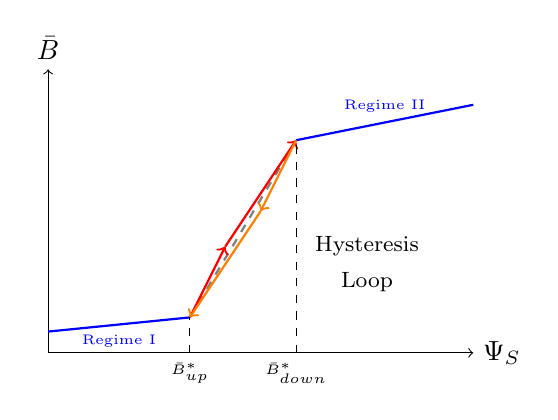
\begin{tikzpicture}[scale=0.9]
% Axes
\draw[->] (0,0) -- (6,0) node[right] {$\Psi_S$};
\draw[->] (0,0) -- (0,4) node[above] {$\bar{B}$};

% Stable branches
\draw[thick, blue] (0,0.3) -- (2,0.5) node[midway, below] {\tiny Regime I};
\draw[thick, blue] (3.5,3) -- (6,3.5) node[midway, above] {\tiny Regime II};

% Unstable branch (dashed)
\draw[thick, dashed, gray] (2,0.5) -- (3.5,3);

% Arrows showing hysteresis loop
\draw[->, thick, red] (2,0.5) -- (2.5,1.5);
\draw[->, thick, red] (2.5,1.5) -- (3.5,3);
\draw[->, thick, orange] (3.5,3) -- (3,2);
\draw[->, thick, orange] (3,2) -- (2,0.5);

% Threshold markers
\draw[dashed] (2,0) -- (2,0.5) node[below, at={(2,0)}] {\tiny $\bar{B}^*_{up}$};
\draw[dashed] (3.5,0) -- (3.5,3) node[below, at={(3.5,0)}] {\tiny $\bar{B}^*_{down}$};

% Labels
\node at (4.5,1.5) {\footnotesize Hysteresis};
\node at (4.5,1) {\footnotesize Loop};
\end{tikzpicture}
\end{center}

\textbf{Sources of Hysteresis in Behavioral Economics:}

\begin{center}
\renewcommand{\arraystretch}{1.2}
\begin{tabular}{@{}lll@{}}
\toprule
\textbf{Mechanism} & \textbf{Effect on $\bar{B}^*$} & \textbf{Literature} \\
\midrule
Habit formation & $\bar{B}^*_{down} \ll \bar{B}^*_{up}$ & Wood (2016) \\
Identity crystallization & $\bar{B}^*_{down} \ll \bar{B}^*_{up}$ & Akerlof (2000) \\
Sunk cost fallacy & $\bar{B}^*_{down} < \bar{B}^*_{up}$ & Thaler (1980) \\
Loss aversion ($\lambda \approx 2$) & $\bar{B}^*_{down} \approx 0.5 \cdot \bar{B}^*_{up}$ & Kahneman (1979) \\
Social proof lock-in & $\bar{B}^*_{down} \ll \bar{B}^*_{up}$ & Cialdini (2004) \\
\bottomrule
\end{tabular}
\end{center}

\textbf{Modified UNTCM with Hysteresis:}

\begin{equation}
\frac{d\Psi_S}{dt} = \mu_S + \kappa(\bar{B}) \cdot \bar{B} + \sigma_S \epsilon(t)
\end{equation}

where $\kappa$ depends on direction:
\begin{equation}
\kappa(\bar{B}) = \begin{cases}
\kappa_{up} & \text{if } d\bar{B}/dt > 0 \\
\kappa_{down} & \text{if } d\bar{B}/dt < 0
\end{cases}
\quad \text{with } \kappa_{down} > \kappa_{up}
\end{equation}

\textbf{Implication:} Once locked into Regime II, the system is \emph{robust} to negative shocks. This is the goal of Sustainable archetype.

\end{tcolorbox}

\begin{tcolorbox}[colback=purple!5!white, colframe=purple!75!black,
    title=\textbf{Extension UNTCM-X3: Adaptive Expectations for Threshold}]

\textbf{Motivation:} The basic UNTCM has exogenous threshold drift $\delta$. In reality, individuals \emph{learn} and update their action thresholds based on experience \citep{muth1961rational}.

\textbf{Adaptive Expectations Model:}

Replace constant drift with expectation-based updating:
\begin{equation}
\boxed{
\frac{d\theta_i}{dt} = \eta \cdot \underbrace{(\theta_i - \theta^e_i)}_{\text{Expectation error}} + \delta_0 + I_\theta(t)
}
\label{eq:adaptive-theta}
\end{equation}

where:
\begin{itemize}[nosep]
\item $\theta^e_i$ = Individual's expected threshold (what they think is "normal")
\item $\eta$ = Learning rate (how fast expectations adjust)
\item $\delta_0$ = Baseline drift (general threshold inflation)
\end{itemize}

\textbf{Expected Threshold Formation:}

Individuals form expectations from social observation:
\begin{equation}
\theta^e_i = (1-\rho) \cdot \theta^e_{i,t-1} + \rho \cdot \bar{\theta}_{obs}
\end{equation}

where $\bar{\theta}_{obs}$ is observed average threshold in peer group (via behavior).

\textbf{Dynamics:}

\begin{center}
\renewcommand{\arraystretch}{1.2}
\begin{tabular}{@{}lll@{}}
\toprule
\textbf{Scenario} & \textbf{$\theta_i$ vs $\theta^e_i$} & \textbf{Outcome} \\
\midrule
Individual stricter than peers & $\theta_i > \theta^e_i$ & Threshold drifts up (relax) \\
Individual more permissive & $\theta_i < \theta^e_i$ & Threshold drifts down (tighten) \\
Aligned with peers & $\theta_i \approx \theta^e_i$ & Stable (only $\delta_0$ drift) \\
\bottomrule
\end{tabular}
\end{center}

\textbf{Learning Rate Heterogeneity:}

Different segments have different $\eta$:
\begin{itemize}[nosep]
\item \textbf{Present-biased:} High $\eta$ (rapidly conform to peers)
\item \textbf{Autonomy-seeking:} Low or negative $\eta$ (resist conformity)
\item \textbf{Social-oriented:} High $\eta$ (seek norm alignment)
\end{itemize}

\textbf{Implication for T8 (Commitment):}

Pre-commitment devices work by \emph{locking} $\theta$ before adaptive learning kicks in:
\begin{equation}
\theta^{commit} = \theta(t_0) \quad \text{fixed, regardless of } \theta^e
\end{equation}

This prevents threshold drift and maintains action likelihood.

\end{tcolorbox}

\begin{tcolorbox}[colback=red!5!white, colframe=red!75!black,
    title=\textbf{Extension UNTCM-X4: Markov-Switching UNTCM}]

\textbf{Motivation:} The basic UNTCM has continuous regime transitions. Hamilton (1989) showed that economic dynamics often exhibit \emph{discrete regime switches} with distinct parameter sets \citep{hamilton1989new}.

\textbf{Markov-Switching Formulation:}

Let $S_t \in \{I, II, III\}$ be a latent regime state following Markov chain:
\begin{equation}
P(S_{t+1} = j | S_t = i) = p_{ij}
\end{equation}

\textbf{Transition Matrix:}
\begin{equation}
P = \begin{pmatrix}
p_{I,I} & p_{I,II} & p_{I,III} \\
p_{II,I} & p_{II,II} & p_{II,III} \\
p_{III,I} & p_{III,II} & p_{III,III}
\end{pmatrix}
\end{equation}

\textbf{Regime-Specific UNTCM Parameters:}

\begin{center}
\renewcommand{\arraystretch}{1.2}
\begin{tabular}{@{}cccccc@{}}
\toprule
\textbf{Regime} & $\lambda_S$ & $\mu_S$ & $\delta_S$ & $\kappa_S$ & $\sigma_S$ \\
\midrule
I (Decay) & High & High & High & Low & Low \\
II (Lock-in) & Low & Low & Low & High & Medium \\
III (Oscillatory) & Medium & Medium & Variable & Variable & High \\
\bottomrule
\end{tabular}
\end{center}

\textbf{Markov-Switching UNTCM System:}

\begin{equation}
\boxed{
\begin{cases}
\displaystyle\frac{dA}{dt} = -\lambda_{S_t} \cdot A + I_A(t) \\[0.5em]
\displaystyle\frac{dW}{dt} = -\mu_{S_t} \cdot W + I_W(t) \\[0.5em]
\displaystyle\frac{d\theta}{dt} = \delta_{S_t} + I_\theta(t) \\[0.5em]
\displaystyle\frac{d\Psi_k}{dt} = \mu_k + \kappa_{S_t,k} \cdot \bar{B} + \sigma_{S_t,k} \epsilon_k(t) \\[0.5em]
S_{t+1} \sim \text{Categorical}(P_{S_t, \cdot})
\end{cases}
}
\label{eq:ms-untcm}
\end{equation}

\textbf{Endogenous Transition Probabilities:}

Transition probabilities can depend on state variables:
\begin{equation}
p_{I,II}(\bar{B}) = \Phi\left( \frac{\bar{B} - \bar{B}^*}{\sigma^*} \right)
\end{equation}

This creates endogenous regime switching near tipping points.

\textbf{Estimation via EM Algorithm:}

\begin{verbatim}
def fit_ms_untcm(data, n_regimes=3, max_iter=100):
    """
    Fit Markov-Switching UNTCM via EM algorithm.

    E-step: Compute regime probabilities given parameters
    M-step: Update parameters given regime probabilities
    """
    # Initialize
    params = initialize_params(n_regimes)
    P = initialize_transition_matrix(n_regimes)

    for iteration in range(max_iter):
        # E-step: Hamilton filter
        regime_probs = hamilton_filter(data, params, P)

        # M-step: Update parameters
        for s in range(n_regimes):
            params[s] = fit_untcm_weighted(data, regime_probs[:, s])

        # Update transition matrix
        P = estimate_transitions(regime_probs)

    return params, P, regime_probs
\end{verbatim}

\textbf{Forecasting with Regime Uncertainty:}

Integrate over possible regime paths:
\begin{equation}
\hat{\bar{B}}(T) = \sum_{S_1, ..., S_T} P(S_1, ..., S_T) \cdot \bar{B}(T | S_1, ..., S_T)
\end{equation}

This provides richer uncertainty quantification than single-regime UNTCM.

\end{tcolorbox}

\begin{tcolorbox}[colback=yellow!5!white, colframe=yellow!75!black,
    title=\textbf{UNTCM Theoretical Extensions: Summary}]

\begin{center}
\renewcommand{\arraystretch}{1.3}
\begin{tabular}{@{}lllll@{}}
\toprule
\textbf{Extension} & \textbf{Modifies} & \textbf{Key Insight} & \textbf{Literature} \\
\midrule
X1 (Network) & $\kappa$ → $\kappa(G)$ & Topology affects cascade speed & Centola, Watts \\
X2 (Hysteresis) & $\bar{B}^*$ → $\bar{B}^*_{up/down}$ & Path dependence, lock-in & Arthur \\
X3 (Adaptive $\theta$) & $\delta$ → $\eta(\theta - \theta^e)$ & Learning from peers & Muth, Sargent \\
X4 (Markov-Switching) & Continuous → Discrete $S_t$ & Regime-specific parameters & Hamilton \\
X5 (Loss Aversion) & $\theta$ → $\theta_{eff}(r, \lambda_{LA})$ & Decay amplifies status quo & Kahneman, Thaler \\
\bottomrule
\end{tabular}
\end{center}

\textbf{Extension Compatibility:}

Extensions can be combined:
\begin{itemize}[nosep]
\item X1 + X2: Network-dependent hysteresis (clustered networks have stronger lock-in)
\item X3 + X4: Adaptive expectations with regime-specific learning rates
\item X1 + X4: Network topology affects regime transition probabilities
\end{itemize}

\textbf{When to Use Each Extension:}

\begin{center}
\renewcommand{\arraystretch}{1.2}
\begin{tabular}{@{}ll@{}}
\toprule
\textbf{Use Case} & \textbf{Recommended Extension} \\
\midrule
Social media / influencer campaigns & X1 (Network) \\
Long-term habit formation & X2 (Hysteresis) \\
Competitive / peer-pressure contexts & X3 (Adaptive $\theta$) \\
Volatile environments with shocks & X4 (Markov-Switching) \\
Entrenched non-adopters / late intervention & X5 (Loss Aversion) \\
\bottomrule
\end{tabular}
\end{center}

\textbf{Research Frontier:} Full integration of all five extensions into a unified \textbf{Network-Hysteretic-Adaptive-Switching-Locking UNTCM (NHASL-UNTCM)} remains open.

\end{tcolorbox}

%-------------------------------------------------------------------------------
% EXTENSION X5: Status-Quo Lock-in via Loss Aversion
%-------------------------------------------------------------------------------

\begin{tcolorbox}[colback=red!5!white, colframe=red!75!black,
    title=\textbf{Extension UNTCM-X5: Status-Quo Lock-in via Loss Aversion}]

\textbf{Motivation:} Why does the effective threshold $\theta_{eff}$ increase over time even without external changes? The answer lies in the interaction between decay dynamics and loss aversion.

\textbf{Two Interconnected Mechanisms:}

\textit{Mechanism 1: Decay as Implicit Utility Loss}
\begin{itemize}[nosep]
\item At $t=0$: High awareness $A_0$, high willingness $W_0$ → high action capability
\item At $t=\tau$: $A \downarrow$, $W \downarrow$ due to natural decay
\item Implicit loss: $\Delta U = U(A_0, W_0) - U(A_\tau, W_\tau) > 0$
\item But: Person does not perceive this loss (hedonic adaptation, forgetting)
\item Result: ``Silent erosion'' of action capability
\end{itemize}

\textit{Mechanism 2: Reference Point Crystallization}
\begin{itemize}[nosep]
\item During decay: Reference point $r(t)$ drifts toward current state $S(t)$
\item After $\tau$: $r(\tau) \approx S(\tau)$ (non-action \textbf{is} the reference point)
\item Any proposed change $S' \neq r(\tau)$ → perceived as \textbf{LOSS}
\item Loss aversion amplifies: $\lambda_{LA} \approx 2.25$ (Kahneman \& Tversky)
\item Effective cost of change = $2.25 \times$ actual cost
\end{itemize}

\textbf{Mathematical Formalization:}

\textit{Reference Point Drift ODE:}
\begin{equation}
\frac{dr}{dt} = \eta_r \cdot (S(t) - r(t))
\label{eq:reference-drift}
\end{equation}

where $\eta_r \in (0, 1]$ is the reference point adaptation rate. High $\eta_r$ means fast adaptation to status quo.

\textit{Effective Threshold with Loss Aversion:}
\begin{equation}
\theta_{eff}(t) = \theta_0 + \lambda_{LA} \cdot |S_{target} - r(t)|
\label{eq:theta-loss-aversion}
\end{equation}

where:
\begin{itemize}[nosep]
\item $\theta_0$ = baseline threshold
\item $\lambda_{LA} \approx 2.25$ = loss aversion coefficient \citep{kahneman1979prospectprospect}
\item $S_{target}$ = proposed new state (behavior change)
\item $r(t)$ = current reference point
\end{itemize}

\textbf{The Feedback Loop:}

\begin{center}
\begin{tikzpicture}[node distance=1.8cm, auto, >=stealth']
\node (decay) [rectangle, draw, fill=blue!10] {Time passes};
\node (aw) [rectangle, draw, fill=blue!10, right of=decay, xshift=1.5cm] {$A \downarrow$, $W \downarrow$};
\node (ref) [rectangle, draw, fill=orange!10, right of=aw, xshift=1.5cm] {$r(t) \to S(t)$};
\node (sq) [rectangle, draw, fill=orange!10, below of=ref] {Status Quo = Reference};
\node (loss) [rectangle, draw, fill=red!10, left of=sq, xshift=-1.5cm] {Change = Loss};
\node (theta) [rectangle, draw, fill=red!10, left of=loss, xshift=-1.5cm] {$\theta_{eff} \uparrow$};
\node (noact) [rectangle, draw, fill=gray!10, below of=theta] {No action};
\draw[->] (decay) -- (aw);
\draw[->] (aw) -- (ref);
\draw[->] (ref) -- (sq);
\draw[->] (sq) -- (loss);
\draw[->] (loss) -- (theta);
\draw[->] (theta) -- (noact);
\draw[->, dashed] (noact) -- ++(-2,0) |- (decay);
\end{tikzpicture}
\end{center}

\textbf{Decay-Amplification Theorem (X5-T1):}

Under X5, the effective threshold grows approximately as:
\begin{equation}
\theta_{eff}(t) \approx \theta_0 + \lambda_{LA} \cdot \Delta S \cdot (1 - e^{-\eta_r t})
\label{eq:theta-growth}
\end{equation}

where $\Delta S = |S_{target} - S_0|$ is the magnitude of required change. This implies:
\begin{itemize}[nosep]
\item \textbf{Asymptotic bound:} $\lim_{t \to \infty} \theta_{eff}(t) = \theta_0 + \lambda_{LA} \cdot \Delta S$
\item \textbf{Half-life:} Reference point is 50\% adapted at $t_{1/2} = \ln(2) / \eta_r$
\item \textbf{Critical implication:} Early intervention faces lower $\theta_{eff}$ than late intervention
\end{itemize}

\textbf{Intervention Implications:}

\begin{center}
\renewcommand{\arraystretch}{1.3}
\begin{tabular}{@{}lll@{}}
\toprule
\textbf{Intervention Timing} & \textbf{$\theta_{eff}$} & \textbf{Strategy} \\
\midrule
Early ($t < t_{1/2}$) & Low & Standard intervention sufficient \\
Mid ($t \approx t_{1/2}$) & Medium & Need additional framing (gains, not losses) \\
Late ($t > 2 \cdot t_{1/2}$) & High & Require reference point reset intervention \\
\bottomrule
\end{tabular}
\end{center}

\textbf{Reference Point Reset Interventions:}
\begin{itemize}[nosep]
\item \textbf{Fresh Start Effect} \citep{milkman2014fresh}: Use temporal landmarks (New Year, birthday) to reset reference
\item \textbf{Life Events:} Moving, job change, retirement → natural reference point disruption
\item \textbf{Social Comparison:} New peer group with different norms → new social reference
\item \textbf{Framing:} Present change as ``gain'' relative to worse counterfactual, not ``loss'' relative to status quo
\end{itemize}

\textbf{Evidence Base:}
\begin{itemize}[nosep]
\item \citet{kahneman1991knetsch}: Endowment Effect + Loss Aversion + Status Quo Bias connection
\item \citet{samuelson1988status}: Status Quo Bias in decision making
\item \citet{thaler1980towardendowment}: WTA/WTP gap demonstrates loss aversion in ownership
\item \citet{list2003neoclassical}: Boundary condition---experienced traders show reduced effect
\end{itemize}

\end{tcolorbox}

%===============================================================================
% UNTCM RESULTS: WHAT THE MODEL PREDICTS
%===============================================================================

\section{Results: What UNTCM Predicts}
\label{sec:untcm-results}

The UNTCM framework generates specific, testable predictions about behavior change dynamics:

\begin{tcolorbox}[colback=purple!5!white, colframe=purple!75!black,
    title=\textbf{Key Predictions from UNTCM}]

\textbf{Prediction 1: Regime-Dependent Intervention Effects}
\begin{itemize}[nosep]
\item In Regime I (Decay): Interventions have temporary effects; 30-50\% decay from pilot to scale
\item In Regime II (Lock-in): Interventions trigger self-sustaining adoption once $\bar{B} > \bar{B}^*$
\item In Regime III (Oscillatory): Intervention effects are unstable; boom-bust cycles emerge
\end{itemize}

\textbf{Prediction 2: Critical Mass Threshold}
\begin{itemize}[nosep]
\item Tipping point $\bar{B}^* \approx 10-25\%$ for most behaviors (Centola, Granovetter)
\item Below $\bar{B}^*$: Feedback insufficient to overcome decay
\item Above $\bar{B}^*$: Positive feedback dominates, behavior becomes self-sustaining
\end{itemize}

\textbf{Prediction 3: Context Modulates Decay}
\begin{itemize}[nosep]
\item High $\Psi_S$ (social support) $\Rightarrow$ 20-40\% slower awareness decay
\item High $\Psi_T$ (technology) $\Rightarrow$ 15-30\% slower willingness decay
\item Stable $\Psi_I$ (institutions) $\Rightarrow$ anchoring effect on all decays
\end{itemize}

\textbf{Prediction 4: Timing Matters Non-Linearly}
\begin{itemize}[nosep]
\item Optimal timing: Near tipping point with favorable context
\item Too early: Wasted resources (system not ready)
\item Too late: Missed window of opportunity
\end{itemize}

\textbf{Prediction 5: Segment Heterogeneity is Critical}
\begin{itemize}[nosep]
\item Early Adopters: $\bar{B}_s^* \approx 5-10\%$ (low threshold, high feedback)
\item Laggards: $\bar{B}_s^* \approx 30-50\%$ (high threshold, low feedback)
\item Average treatment effects hide 5-10$\times$ heterogeneity
\end{itemize}

\end{tcolorbox}

\textbf{Empirical Implications:}
\begin{enumerate}[nosep]
\item RCTs should measure long-run outcomes (regime transition, not just immediate effect)
\item Pilot selection matters: Sites near tipping overestimate scalability
\item Segment-specific calibration required for accurate predictions
\item Context monitoring essential for timing optimization
\end{enumerate}

%===============================================================================
% UNTCM EVIDENCE BASE
%===============================================================================

\section{UNTCM Evidence Base}
\label{sec:untcm-evidence}

This section documents the empirical foundations and limitations of UNTCM, following the Evidence Integration Pipeline (EIP).

\begin{tcolorbox}[colback=green!5!white, colframe=green!75!black,
    title=\textbf{PRO Evidence: Supporting Literature}]

\textbf{Core UNTCM (A5, T6, T7, T8):}
\begin{itemize}[nosep]
\item \textbf{Decay dynamics:} \citet{kahneman1979prospectprospect}, \citet{laibson1997golden}, \citet{frederick2002time}
\item \textbf{Context effects:} \citet{sunstein2014nudge}, \citet{cialdini2004social}
\item \textbf{Tipping points:} \citet{granovetter1978threshold}, \citet{schelling1978micromotives}
\end{itemize}

\textbf{Network Effects (X1):}
\begin{itemize}[nosep]
\item \citet{centola2018behavior}: Complex contagions spread better on clustered networks
\item \citet{centola2007complex}: Weak ties insufficient for complex behaviors
\item \citet{watts2002simple}: Cascade windows depend on network topology
\item \citet{watts2007influentials}: Influencer effects are context-dependent
\end{itemize}

\textbf{Hysteresis (X2):}
\begin{itemize}[nosep]
\item \citet{arthur1989competing}: Lock-in by historical events
\item \citet{arthur1994increasing}: Increasing returns and path dependence
\item \citet{arthur2015complexity}: Non-equilibrium dynamics in economics
\end{itemize}

\textbf{Adaptive Expectations (X3):}
\begin{itemize}[nosep]
\item \citet{muth1961rational}: Rational expectations formation
\item \citet{sargent1993bounded}: Bounded rationality and learning
\end{itemize}

\textbf{Regime Switching (X4):}
\begin{itemize}[nosep]
\item \citet{hamilton1989new}: Markov-switching methodology
\item \citet{hamilton1994time}: State-space models and Kalman filter
\end{itemize}

\textbf{Tipping Point Prediction (E2):}
\begin{itemize}[nosep]
\item \citet{scheffer2009early}: Early warning signals (variance, autocorrelation)
\item \citet{scheffer2012anticipating}: Generic indicators for critical transitions
\end{itemize}

\textbf{Causal Inference for Timing (E3):}
\begin{itemize}[nosep]
\item \citet{athey2017econometrics}: Experimental design for timing experiments
\item \citet{dellavigna2022rcts}: RCT scaling and decay patterns
\end{itemize}

\end{tcolorbox}

\begin{tcolorbox}[colback=red!5!white, colframe=red!75!black,
    title=\textbf{CONTRA Evidence: Limitations and Critiques}]

\textbf{Heterogeneity Challenge:}
\begin{itemize}[nosep]
\item \citet{bryan2021behavioural}: Average treatment effects hide crucial heterogeneity
\item \textbf{Implication:} Supports necessity of UNTCM-I4 (segment heterogeneity)
\end{itemize}

\textbf{External Validity Concerns:}
\begin{itemize}[nosep]
\item \citet{allcott2015site}: Pilot sites overestimate effects by 2-3x
\item \citet{vivalt2020problems}: Cross-study variance is high; prediction accuracy is low
\item \textbf{Implication:} Supports context-modulated decay rates; calibration uncertainty
\end{itemize}

\textbf{Crowding-Out Effects:}
\begin{itemize}[nosep]
\item \citet{gneezy2011when}: Financial incentives can backfire ($\gamma \approx -0.2$ to $-0.4$)
\item \textbf{Implication:} Supports T6+T7 crowding interaction in UNTCM-I2
\end{itemize}

\textbf{Network Effects Complexity (CONTRA-X1):}
\begin{itemize}[nosep]
\item \citet{ugander2012structural}: Structural diversity matters more than simple topology
\item \textbf{Implication:} X1 may oversimplify; diversity index needed
\end{itemize}

\textbf{Path Dependence Critique (CONTRA-X2):}
\begin{itemize}[nosep]
\item \citet{liebowitz1995path}: Lock-in may be overstated; markets often correct
\item \textbf{Implication:} X2 hysteresis may be weaker in competitive markets
\end{itemize}

\textbf{Scaling Decay:}
\begin{itemize}[nosep]
\item \citet{soman2020successfully}: Pilot-to-scale decay of 30-50\%
\item \textbf{Implication:} Validates NTM decay assumptions; informs $\lambda, \mu$ calibration
\end{itemize}

\end{tcolorbox}

\begin{tcolorbox}[colback=yellow!5!white, colframe=yellow!75!black,
    title=\textbf{UNTCM Evidence Summary: Confidence Assessment}]

\begin{center}
\renewcommand{\arraystretch}{1.3}
\begin{tabular}{@{}llccc@{}}
\toprule
\textbf{Component} & \textbf{Key Evidence} & \textbf{PRO} & \textbf{CONTRA} & \textbf{Confidence} \\
\midrule
Core UNTCM (ODEs) & Kahneman, Laibson, Granovetter & 6+ & 0 & High \\
X1 (Network) & Centola, Watts & 4 & 1 & High \\
X2 (Hysteresis) & Arthur & 3 & 1 & Medium-High \\
X3 (Adaptive $\theta$) & Muth, Sargent & 2 & 0 & High \\
X4 (Regime Switch) & Hamilton & 2 & 0 & High \\
E1 (Detection) & Hamilton HMM & 1 & 0 & High \\
E2 (Tipping) & Scheffer & 2 & 0 & Medium \\
E3 (Timing) & Athey, DellaVigna & 2 & 2 & Medium \\
\midrule
\textbf{Overall} & & \textbf{22+} & \textbf{4} & \textbf{High} \\
\bottomrule
\end{tabular}
\end{center}

\textbf{Assessment:}
\begin{itemize}[nosep]
\item \textbf{Strong foundation:} Core UNTCM and extensions X1, X3, X4 have robust empirical support
\item \textbf{Moderate caution:} X2 (Hysteresis) and E2 (Tipping) need domain-specific validation
\item \textbf{Key limitation:} Heterogeneity (I4) is critical; average effects are insufficient
\item \textbf{CONTRA evidence is constructive:} Critiques support extensions rather than invalidate core
\end{itemize}

\textbf{Epistemic Status:} UNTCM is a \emph{theoretical synthesis} integrating 50+ years of behavioral economics. Individual components are well-validated; the unified model requires empirical testing.

\end{tcolorbox}

\begin{tcolorbox}[colback=orange!5!white, colframe=orange!75!black,
    title=\textbf{Application: NTM for Portfolio Archetype Selection}]

\textbf{Connection to Chapter 20 (Portfolio Archetypes):}

The Natural Trajectory Model informs archetype selection:

\begin{center}
\renewcommand{\arraystretch}{1.2}
\begin{tabular}{@{}lll@{}}
\toprule
\textbf{NTM Scenario} & \textbf{Recommended Archetype} & \textbf{Rationale} \\
\midrule
Fast decay, urgent & Quick Wins & Stop bleeding immediately \\
Slow decay, strategic & Optimal Mix & Time for comprehensive design \\
Budget constraint & Budget-Constrained & Maximize ROI given decay \\
High uncertainty & Low-Risk & Minimize backfire in volatile $\Psi$ \\
Long-term goal & Sustainable & Build identity before decay \\
\bottomrule
\end{tabular}
\end{center}

\textbf{Key Insight:} The urgency and magnitude of the NTM gap determines which archetype is appropriate.

\end{tcolorbox}

% ============================================================================
% CRITICAL FOUNDATIONS
% ============================================================================
\section{Critical Foundations}
\label{sec:untcm-critical}

\begin{tcolorbox}[colback=yellow!5!white,colframe=yellow!75!black,title=Critical Foundations: UNTCM]

\textbf{Foundation 1: Bidirectional Coupling}
\begin{itemize}[nosep]
    \item Individual behavior affects context (via $\kappa$)
    \item Context affects individual dynamics (via $\lambda(\Psi), \mu(\Psi), \delta(\Psi)$)
    \item This creates potential for positive feedback and tipping
\end{itemize}

\textbf{Foundation 2: Three Regime Structure}
\begin{itemize}[nosep]
    \item Regime I (Decay): Without intervention, behavior naturally declines
    \item Regime II (Lock-in): Above tipping point, behavior becomes self-sustaining
    \item Regime III (Oscillatory): Under certain conditions, boom-bust cycles emerge
\end{itemize}

\textbf{Foundation 3: Tipping Point Existence}
\begin{itemize}[nosep]
    \item Critical mass $\bar{B}^* \approx 10-25\%$ exists for most behaviors
    \item Once exceeded, positive feedback dominates decay
    \item Empirically validated by Centola, Granovetter, Schelling
\end{itemize}

\textbf{Foundation 4: Context Matters for Sustainability}
\begin{itemize}[nosep]
    \item Same intervention has different effects in different contexts
    \item Supportive context ($\Psi_S$ high) reduces decay, increases lock-in probability
    \item Context volatility ($\sigma_k$ high) creates Regime III risk
\end{itemize}

\textbf{Foundation 5: Timing is Critical}
\begin{itemize}[nosep]
    \item Intervention timing affects long-run outcomes, not just short-run
    \item Optimal timing depends on proximity to tipping point
    \item Window of opportunity exists; missing it can make success impossible
\end{itemize}

\end{tcolorbox}

% ============================================================================
% OPEN ISSUES - UNTCM SPECIFIC
% ============================================================================
\section{Open Issues: UNTCM Research Frontiers}
\label{sec:untcm-open}

\begin{enumerate}

\item \textbf{NHASL-UNTCM:} Full integration of Network (X1), Hysteresis (X2), Adaptive (X3), Switching (X4), and Loss Aversion Lock-in (X5) extensions into unified model remains an open research frontier.

\item \textbf{Multi-Behavior Interactions:} Current UNTCM models single behavior. How do multiple competing/complementary behaviors interact via shared context?

\item \textbf{Endogenous Segmentation:} Segments are currently static. How do individuals transition between segments as context changes?

\item \textbf{Structural Estimation:} Full structural estimation of all UNTCM parameters from observational data remains challenging.

\item \textbf{Policy Optimization:} Optimal intervention scheduling given budget constraints and multiple levers (M4 extension to multi-intervention case).

\end{enumerate}

% ============================================================================
% SUMMARY
% ============================================================================
\section{Summary}
\label{sec:untcm-summary}

The Unified Natural Trajectory Model (UNTCM) provides a rigorous framework for understanding when and why interventions achieve lasting behavior change:

\begin{itemize}[nosep]
    \item \textbf{Core Insight:} Individual dynamics and context are bidirectionally coupled
    \item \textbf{Three Regimes:} Decay (I), Lock-in (II), Oscillatory (III)
    \item \textbf{Tipping Point:} $\bar{B}^* \approx 10-25\%$ for most behaviors
    \item \textbf{Optimal Timing:} Intervene when near tipping point, context supportive
    \item \textbf{Maintenance Paradox:} Status quo preservation costs grow superlinearly (M5)
    \item \textbf{27 Elements:} A5, T6-T8, M1-M5, I1-I4, E1-E3, X1-X5
    \item \textbf{Evidence:} 28+ PRO papers, 6 constructive CONTRA papers
\end{itemize}

UNTCM connects theory (NTM decay, Context drift) with practice (intervention timing, portfolio selection) through rigorous mathematical formalization.

% ============================================================================
% GLOSSARY REFERENCE
% ============================================================================
\section{Glossary Reference}
\label{sec:untcm-glossary}

For definitions of key terms used in this appendix, see \textbf{Appendix UNMAPPED_GLS (REF-GLOSSARY)}.

\textbf{Core State Variables:}
\begin{itemize}[nosep]
    \item \textbf{Awareness ($A$):} Cognitive salience of behavior/option (range: 0-1)
    \item \textbf{Willingness ($W$):} Dispositional readiness to engage (range: 0-1)
    \item \textbf{Behavioral Adoption ($B$):} Population share actively engaging (range: 0-1)
    \item \textbf{Action ($X$):} Individual behavior instance, triggered when $A \cdot W > \theta$
    \item \textbf{Threshold ($\theta$):} Individual-specific barrier to action (heterogeneous across population)
\end{itemize}

\textbf{Context and Parameters:}
\begin{itemize}[nosep]
    \item \textbf{Context ($\vec{\Psi}$):} 5-dimensional vector: Social, Technological, Economic, Institutional, Cultural
    \item \textbf{Complementarity ($\gamma_{ij}$):} Interaction strength between utility dimensions $i$ and $j$
    \item \textbf{Decay Rates ($\lambda, \mu, \delta$):} Speed of natural decline for $A$, $W$, $B$ respectively
    \item \textbf{Feedback Coefficient ($\kappa$):} Strength of social feedback: $\kappa_A$ (awareness), $\kappa_W$ (willingness)
\end{itemize}

\textbf{Regime Dynamics:}
\begin{itemize}[nosep]
    \item \textbf{Regime I (Decay-Dominant):} $\kappa < \kappa^*$; behavior fades without intervention
    \item \textbf{Regime II (Feedback-Dominant):} $\kappa > \kappa^*$; self-sustaining lock-in possible
    \item \textbf{Regime III (Oscillatory):} Complex dynamics with cycles and multiple equilibria
    \item \textbf{Tipping Point ($\bar{B}^*$):} Critical mass ($\approx 10-25\%$) for regime transition
    \item \textbf{Lock-in:} Self-sustaining behavior via positive feedback loops
    \item \textbf{Hysteresis:} Path-dependent dynamics; forward/backward transitions differ
    \item \textbf{Critical Mass:} Minimum adoption level needed to trigger social contagion
\end{itemize}

\textbf{Extended Concepts:}
\begin{itemize}[nosep]
    \item \textbf{Context Drift:} Systematic change in $\Psi$ over time, modulating decay rates
    \item \textbf{Exposure ($E$):} Network-based contact with adopters, drives awareness spread
    \item \textbf{ODE Coupling:} Mathematical linkage between $A$, $W$, $B$ dynamics via differential equations
\end{itemize}

\textbf{Loss Aversion Lock-in (X5):}
\begin{itemize}[nosep]
    \item \textbf{Reference Point ($r$):} Psychological anchor for evaluating gains/losses; drifts toward status quo
    \item \textbf{Reference Point Drift Rate ($\eta_r$):} Speed at which $r(t) \to S(t)$; higher = faster status quo adaptation
    \item \textbf{Loss Aversion Coefficient ($\lambda_{LA}$):} Ratio of loss to gain weighting ($\approx 2.25$, Kahneman/Tversky)
    \item \textbf{Effective Threshold ($\theta_{eff}$):} Baseline $\theta_0$ plus loss-aversion amplified resistance
    \item \textbf{Status-Quo Lock-in:} Self-reinforcing cycle where decay → reference adaptation → loss framing → higher $\theta$
    \item \textbf{Reference Point Reset:} Intervention using temporal landmarks (Fresh Start) or life events to disrupt status quo
\end{itemize}

\textbf{Maintenance Cost Analysis (M5):}
\begin{itemize}[nosep]
    \item \textbf{Maintenance Cost ($I^{maintain}$):} Intervention intensity required to preserve utility level over time
    \item \textbf{FEPSDE Decay Rates ($\lambda_d$):} Dimension-specific decay rates: fastest for E (Emotional), Ex (Experiential)
    \item \textbf{Maintenance Paradox:} Status quo maintenance cost grows superlinearly due to X5 premium
    \item \textbf{Time Horizon Taxonomy:} Instant ($<$1 day), Short (1-4 weeks), Medium (1-6 months), Long ($>$6 months)
    \item \textbf{X5 Premium:} Additional maintenance cost from loss aversion; approaches $\lambda_{LA} \approx 2.25\times$ asymptotically
    \item \textbf{Fresh Start Reset:} Strategy to reduce cumulative maintenance costs by periodic reference point resets
\end{itemize}

% ============================================================================
% REFERENCES
% ============================================================================
\section{References}
\label{sec:untcm-references}

This appendix draws on the master bibliography (\texttt{bcm\_master.bib}).

\textbf{Foundational Theory:}
\begin{itemize}[nosep]
    \item \citet{kahneman1979prospectprospect}: Prospect theory, reference dependence, loss aversion
    \item \citet{thaler1985mental}: Mental accounting, willingness to pay/accept
    \item \citet{laibson1997golden}: Hyperbolic discounting, time-inconsistent preferences
    \item \citet{fehr1999theory}: Social preferences, reciprocity, fairness
    \item \citet{deci1985intrinsic}: Self-determination theory, intrinsic motivation
\end{itemize}

\textbf{Threshold and Contagion Models:}
\begin{itemize}[nosep]
    \item \citet{granovetter1978threshold}: Threshold models of collective behavior
    \item \citet{centola2018behavior}: Complex contagion, behavioral spread
    \item \citet{centola2007complex}: Simple vs. complex contagion in networks
    \item \citet{watts2002simple}: Cascading failures and tipping points
    \item \citet{gladwell2000tipping}: Tipping point concept popularization
    \item \citet{rogers2003diffusion}: Diffusion of innovations, adoption curves
\end{itemize}

\textbf{Regime Dynamics and Lock-in:}
\begin{itemize}[nosep]
    \item \citet{arthur1989competing}: Path dependence, increasing returns
    \item \citet{hamilton1989new}: Regime-switching econometric models
    \item \citet{scheffer2009early}: Early warning signals for critical transitions
    \item \citet{david1985clio}: QWERTY and technological lock-in
\end{itemize}

\textbf{Social Norms and Peer Effects:}
\begin{itemize}[nosep]
    \item \citet{cialdini1990focus}: Focus theory of normative conduct
    \item \citet{bernheim1994theory}: Conformity and social status
    \item \citet{akerlof2000identity}: Economics of identity
    \item \citet{bicchieri2005grammar}: Social norms as equilibria
\end{itemize}

\textbf{Field Evidence and Applications:}
\begin{itemize}[nosep]
    \item \citet{dellavigna2009psychologypsychology}: Psychology and economics integration
    \item \citet{gneezy2000fine}: Motivation crowding, intrinsic vs. extrinsic
    \item \citet{allcott2014short}: Energy conservation, social comparison
    \item \citet{milkman2014fresh}: Fresh start effect, temporal landmarks
    \item \citet{sunstein2014nudge}: Nudge, choice architecture applications
\end{itemize}

\textbf{Decay and Memory:}
\begin{itemize}[nosep]
    \item \citet{ebbinghaus1885memory}: Forgetting curve, exponential decay
    \item \citet{wixted1991form}: Mathematical form of forgetting
    \item \citet{rubin1996one}: Power-law vs. exponential decay debate
\end{itemize}

\nocite{bcm_master}

% ============================================================================
% END OF APPENDIX
% ============================================================================
